%%%%%%%%%%%%%%%%%%%% book_it.tex %%%%%%%%%%%%%%%%%%%%%%%%%%%%%
%
% Esempio di file principale per i capitoli della vostra  "monografia"
%
% Usare questo file come template per il vostro documento.
%
%%%%%%%%%%%%%%%% Springer-Verlag %%%%%%%%%%%%%%%%%%%%%%%%%%


% CONSIGLIATO
%%%%%%%%%%%%%%%%%%%%%%%%%%%%%%%%%%%%%%%%%%%%%%%%%%%
\documentclass[envcountsame,envcountchap]{svmono}

% scegliere le opzioni per []  come richiesto dalla lista 
% nella Reference Guide, Sez. 2.2

\usepackage{makeidx}         % permette di generare l'indice
\usepackage{graphicx}        % pacchetto grafico standard LaTeX 
                             % per l'inclusione di file immagine
\graphicspath{{./}{Figure/}}
\usepackage{multicol}        % usato per l'indice a due colonne
\usepackage[bottom]{footmisc}% mette le note a pie' di pagina
\usepackage[italian]{babel}
\usepackage[utf8]{inputenc}
\usepackage[T1]{fontenc}
\usepackage{amsmath}
\usepackage{amssymb}
\usepackage{graphicx}
\usepackage{epstopdf}
\usepackage[svgpath=./Figure/]{svg}
\usepackage{mathtools}
\usepackage{cite}
\usepackage{placeins}
\include{BibMBS.bib}

% etc.
% si veda la lista di ulteriori pacchetti utili 
% nella Reference Guide, Sez. 2.3, 3.1-3.3

\def\theoremname{Teorema}
\makeindex             % usato per l'indice degli argomenti 
                       % si prega di usare lo stile svind.ist con 
                       % il vostro programma makeindex

\def\avect#1{{\boldsymbol{#1}}}
\def\amatr#1{{\boldsymbol{#1}}}
\newcommand{\norm}[1]{\left\lVert#1\right\rVert}
%%%%%%%%%%%%%%%%%%%%%%%%%%%%%%%%%%%%%%%%%%%%%%%%%%%%%%%%%%%%%%%%%%%%%

\begin{document}

\author{Simone Benatti}
\title{Metodi numerici per la soluzione del problema di Cauchy nelle simulazioni Multibody
%{\small SPIN Springer internal project number, se noto}
}
\subtitle{Elaborato Finale di Matematica Numerica \newline proff.sa A. Aimi \newline AA 2017/2018}
\date{Giugno 2018}
\maketitle

\frontmatter%%%%%%%%%%%%%%%%%%%%%%%%%%%%%%%%%%%%%%%%%%%%%%%%%%%%%%

%\include{Contenuto/dedic_it}
%\include{Contenuto/pref_it}

\tableofcontents


\mainmatter%%%%%%%%%%%%%%%%%%%%%%%%%%%%%%%%%%%%%%%%%%%%%%%%%%%%%%%
%%%%%%%%%%%%%%%%%%%%%%%% part.tex %%%%%%%%%%%%%%%%%%%%%%%%%%%%%%%%%%
%
% esempio di titolo della parte
%
% Usare questo file come template per il vostro documento.
%
%%%%%%%%%%%%%%%%%%%%%%%% Springer-Verlag %%%%%%%%%%%%%%%%%%%%%%%%%%


\part{Dinamica Lagrangiana}\label{part:LagrDyn}

%%%%%%%%%%%%%%%%%%%%% chapter.tex %%%%%%%%%%%%%%%%%%%%%%%%%%%%%%%%%
%
% esempio di capitolo
%
% Usare questo  file come template per il vostro documento.
%
%%%%%%%%%%%%%%%%%%%%%%%% Springer-Verlag %%%%%%%%%%%%%%%%%%%%%%%%%%

\chapter{Rotazioni}
\label{Rotazioni} % Fornire sempre un'unica label
% usare \chaptermark{}
% per alterare o aggiustare l'intestazione del capitolo nella running head

Trasformazioni di un vettore utilizzando angoli di rotazione o quaternioni.
\section{Matrice di rotazione}
Con la matrice di rotazione $[_1^0A]$ si intende la matrice che trasforma le coordinate del vettore r espresse nel riferimento ruotato 1 ${^1r}$ , nel sistema di riferimento 0. \newline In generale sarà presente anche una traslazione tra i due riferimenti, ragion per cui compare un termine di traslazione d:
\begin{equation}
\label{eq:1.1}
\left\{^0r\right\} = \left[_1^0A\right]\left\{^1r\right\} + \left\{^0d\right\}
\end{equation}

\begin{figure}[h!]
\centering
\includegraphics[height=6cm]{rotation_1.png}
\caption{Trasformazione delle coordinate di un punto}
\label{fig:1.1}
\end{figure}
La matrice di rotazione $\in \mathbb{R}^{3x3}$ per cui è definita da 9 elementi, tuttavia per calcolarla bastano 3 o 4 parametri a seconda che si utilizzino gli angoli di rotazione o i quaternioni.
\section{Angoli di Eulero}
La matrice relativa alla rotazione attorno ad un asse del riferimento può essere ricavata con calcoli trigonometrici. Poiché una qualsiasi rotazione può essere espressa come una successione di 3 rotazioni attorno a 3 assi distinti è possibile risalire alla coordinata del punto nel riferimento 3 arbitrariamente ruotato con un prodotto di matrici:
\begin{equation}
\label{eq:1.2}
\left\{^0r\right\} = \left[_1^0A\right]\left[_2^1A\right]\left[_3^2A\right]\left\{^3r\right\}
\end{equation}
La scelta della sequenza di assi di rotazione non è univoca. Per questo si sono diffuse differenti convenzioni. La più diffusa è quella degli angoli di Eulero:
\begin{figure}[h!]
\centering
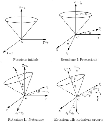
\includegraphics[height=10cm]{euler_angles.pdf}
\caption{Angoli di Eulero}
\label{fig:1.2}
\end{figure}
L'utilizzo della matrice di rotazione fornisce formule dirette per il calcolo di posizioni, velocità ed accelerazioni nel riferimento fisso a patto di conoscere angoli e velocità angolari dei sistemi di riferimento solidali ai corpi del sistema. Emergono tuttavia due limiti a questo approccio: \begin{itemize}
\item L'ordine di applicazione degli angoli di rotazione dà luogo a configurazioni finali differenti (d'altronde il prodotto tra matrici non è commutativo). L'influenza dell'ordine di applicazione degli angoli ha portato diversi enti ad adottare diverse convenzioni.
\item Il limite maggiore di questo approccio tuttavia è l'emergere di singolarità nella soluzione del problema inverso; ovvero qualora si vogliano trovare gli angoli a partire dalla matrice, problema molto comune nelle applicazioni robotiche. Formalmente, esprimendo con x', y' e z' i versori lungo gli assi del riferimento mobile (ovviamente rispetto a quello fisso), si devono eguagliare elemento per elemento le matrici
\[ \begin{bmatrix}   \\ x'& y'&z' \\ \text{ } \end{bmatrix} = \begin{bmatrix}
a_{11} & a_{12} & a_{13} \\ a_{21} & a_{22} & a_{23} \\ a_{31} & a_{32} & a_{33}\end{bmatrix} \]
Con: \qquad $a_{33} = cos\theta,\qquad a_{32} = -sin\theta cos\phi \qquad$ ecc... \newline
È evidente che in corrispondenza di certi angoli si riscontrano singolarità ad è impossibile risolvere il sistema di 9 equazioni. Questo ha anche un riscontro pratico detto blocco cardanico o \textit{gimbal lock}: una sospensione cardanica con 3 cerniere con lo scopo di isolare un oggetto dalle rotazioni del telaio in certe configurazioni non permette più rotazioni arbitrarie, di fatto bloccando alcune rotazioni.  
\end{itemize}

\section{Quaternioni}
Per questa ragione si utilizzano 4 parametri, descrivendo le rotazioni tramite quaternioni. Si evitano così le singolarità nella cinematica inversa, l'utilizzo di funzioni trigonometriche per la soluzione del sistema ed il problema dell'arbitrarietà della sequenza di rotazioni.
In Generale un quaternione è un elemento scrivibile come $ \overline{q} = a + bi + cj+ ck$ con $i^2=j^2=k^2 = ijk -1$. \newline Il quaternione descrive una rotazione di un angolo $\theta$ attorno ad un versore u come in figura \ref{fig:1.3}.

La rotazione di un angolo $\theta$ attorno ad un versore di componenti ${a, b, c}$ è quindi decritta dal quaternione
\begin{equation} 
    \overline{q} = cos\frac{\theta}{2} + (ai + bj + ck)sin\frac{\theta}{2}
\end{equation}{}

Tramite l'utilizzo dei quaternioni si può esprimere:
\begin{itemize}
\item La cinematica diretta \begin{equation}
\label{eq:1.3}
(0, v') = \overline{q}(0,v)\overline{q}^*\end{equation}
Con (0,v) vettore di 4 elementi e $\overline{q}^*$ coniugato di $\overline{q}$
\item La cinematica inversa: \begin{equation}
\label{eq:1.4}
(0, v) = \overline{q}^*(0,v')\overline{q}\end{equation}
\item Rotazioni successive :
\begin{equation} 
    \overline{q} = \overline{q}_2 \overline{q}_1 
\end{equation}{}
\item La matrice di rotazione A:
\begin{equation}\left[A(q)\right] = \left[F(q)_+\right]\left[F(q)_-\right]^T \label{eq:1.5}\end{equation}
Con 
\begin{equation} \label{eq:1.6} \left[F(q)_+\right]\ = \begin{bmatrix}
+q_1 & +q_0 & -q_3 & +q_2 \\ +q_2 & +q_3 & +q_0 & -q_1 \\ +q_3 & -q_2 & +q_1 &+q_0\end{bmatrix}
\end{equation}
\begin{equation} \label{eq:1.7} \left[F(q)_-\right]\ = \begin{bmatrix}
+q1 & +q_0 & +q_3 & -q_2 \\ +q_2 & -q_3 & +q_0 & +q_1 \\ +q_3 & +q_2 & -q_1 &+q_0\end{bmatrix}
\end{equation}
\item Velocità in funzione di $ \dot{\overline{q}}$ e viceversa
\begin{equation} \label{eq:1.8}
\dot{\overline{q}} = \frac{1}{2}\left[F(q^*)_-\right]\overrightarrow{\omega}_0 = \frac{1}{2}\left[F(q^*)_+\right]\overrightarrow{\omega}_l\end{equation}
\begin{equation} \label{eq:1.9}
\overrightarrow{\omega}_0 = 2\left[F(q^*)_-\right]\dot{\overline{q}}\end{equation}
\begin{equation} \label{eq:1.10}
\overrightarrow{\omega}_l = 2\left[F(q^*)+-\right]\dot{\overline{q}}\end{equation}
\item Accelerazione angolare in funzione di $\ddot{\overline{q}}$ e viceversa
\end{itemize}
\begin{figure}[h!]
\centering
\includegraphics[height=5cm]{quaternion_def.png}
\caption{Trasformazione delle coordinate di un punto}
\label{fig:1.3}
\end{figure}




%


\chapter{Formula di Lagrange}
\label{Formula di Lagrange} 
%\textbf{Nota:} Per facilitare la lettura in seguito si userà il grassetto per le quantità vettoriali mentre l'overline indicherà che le coordinate in questione sono relative. \newline
\section{Lavoro Virtuale}
Un passaggio essenziale nella formulazione lagrangiana delle equazioni della dinamica del sistema multibody è il calcolo delle forze generalizzate associate con le forze generalizzate del sistema.
In questa sezione le forze generalizzate sono introdotte applicando il principio dei lavori virtuali nei casi statico e dinamico. Nello svolgimento in seguito si considera un sistema di particelle.
Assumendo che un corpo rigido non è altro che un grande numero di particelle queste espressioni saranno estese ai corpi rigidi con poche modifiche.
\paragraph{Equilibrio Statico}
Si consideri un sistema composto da $n_p$ particelle. Se il sistema di particelle è in equilibrio significa che 
\begin{equation}
\label{eq:equilibrium_virtualwork}
\mathbf{ \sum_{i=1}^{n_p} F^i \delta r^i }=  0
\end{equation}
Dove F ed r sono la forza agente e lo spostamento virtuale relativi ad un particella i. La forze sono di 2 tipi: forze esterne e forze di vincolo: 
$F^i_e +F^i_c = F^i$ ed applicando questa suddivisione all'equazione \ref{eq:equilibrium_virtualwork} si ottiene:
\[\sum_{i=1}^{n_p}F^i\delta r^i = 0 \Rightarrow \sum_{i=1}^{n_p}F_e^i\delta r^i + \sum_{i=1}^{n_p}F_c^i\delta r^i = 0 \Rightarrow \delta W_e + \delta W_c = 0 \]
Lo spostamento di ogni particella è funzione delle coordinate del sistema $q= (q_1, q_2,\quad ... \quad q_n)$.
\[r_i = r_i(q_1, q_2,\quad ... \quad q_n) \Rightarrow \delta r_i = 
\frac{\partial r_i}{\partial q_1}\delta q_1 + \frac{\partial r_i}{\partial q_2}\delta q_2 + \frac{\partial r_i}{\partial q_3}\delta q_3 + .... + \frac{\partial r_i}{\partial q_n}\delta q_n \]
Si consideri il caso in cui i vincoli non compiono lavoro (\emph{workless constraints}), ad esempio quando i vincoli non hanno attrito (o la forza di attrito viene inserita fra le forze esterne). In questo caso il lavoro virtuale è dovuto alle sole forze esterne: \begin{equation}
\delta W = \delta W _e = 
\sum_{i=1}^{n_p}\left( F_e^i \sum_{j=1}^n \frac{\partial r_i}{\partial q_j}\delta q_j \right) = 0
\end{equation}
Si definisce $Q_j$ come: \begin{equation}
Q_j = \sum_{i=1}^n F_e^i \frac{\partial r_i}{\partial q_j} = \sum_{i=1}^n \left(F_e^i\right)^T r^i_{q_j} \qquad \left( r^i_{q_j}=\frac{\partial r_i}{\partial q_j} \right)
\end{equation}
Per cui si ottiene: \begin{equation}
\delta W = \delta W_e = \sum_{j=1}^n Q_j\delta q_j = Q^T \delta q = 0
\end{equation}
Con \begin{equation}
Q = \left[Q_1, Q_2 , .... , Q_n\right]^T
\end{equation}
Vettore delle forze generalizzate.

\paragraph{Equilibrio dinamico, Principio di D'Alembert}
La seconda legge di Newton afferma che: \begin{equation}
\label{eq:newton_law}
F^i = \dot{P}^i \qquad o \qquad F^i - \dot{P}^i = 0
\end{equation}
Con F risultante delle forze e P quantità di moto agenti sulla generica particella i. 
Da \ref{eq:newton_law} esplicitando il lavoro virtuale di un sistema di particelle in equilibrio dinamico si 
ottiene il \emph{principio di D'Alembert}
\begin{gather} 
\label{eq:dalembert_principle}
\sum_{i=1}^{n_p} (F_e^i + F_c^i -\dot{P}^i )\delta r^i = \sum_{i=1}^{n_p} (F_e^i -\dot{P}^i )\delta r^i + \sum_{i=1}^{n_p} F_c^i\delta r^i = 0 \nonumber \\ \underset{workless constraints}{\Rightarrow} \sum_{i=1}^{n_p} (F_e^i -\dot{P}^i )\delta r^i = 0 \nonumber \\ \Rightarrow \sum_{i=1}^{n_p} (F_e^i -\dot{P}^i )\sum_{j=1}^n \frac{\partial r_i}{\partial q_j} \delta q_j = 0
\end{gather}

Ridefinendo $Q_j$ nel caso dinamico comprendendo il contributo delle forze d'inerzia si ottiene:
\begin{equation}
Q_j = \sum_{i=1}^{n_p} \left(F_e^i-\dot{P}^i\right)\frac{\partial r^i}{\partial q_j}
\end{equation}
Da cui:
\begin{equation}
\sum_{j=1}^n \sum_{i=1}^{n_p} \left(F_e^i-\dot{P}^i\right)\frac{\partial r^i}{\partial q_j}\delta q_j = \sum_{j=1}^n Q_j \delta q_j = Q^T = 0
\end{equation}
\section{Dinamica Lagrangiana per particelle}
Si introduce qui la formulazione lagrangiana della dinamica di un sistema di particelle che verrà in seguito estesa
ai corpi rigidi.
\subsection{Lavoro Virtuale su un sistema di particelle}
\paragraph{Spostamento di una particella \emph{i}}
Lo spostamento di una particella \emph{r} è funzione del sistema di coordinate \emph{q} e del tempo \emph{t}:
\begin{equation}
r^i = r^i\left(q_1, q_2, q_3 ... ,q_n, t\right)
\end{equation}
Da cui si ottiene, derivando a catena:
\begin{align}
\label{eq:particle_disp_time_der}
\dot{r}^i = \frac{D r^i}{D t} & = \frac{\partial r^i}{\partial q_1}\dot{q_1} + \frac{\partial r^i}{\partial q_2}\dot{q_2}
+ ... + \frac{\partial r^i}{\partial q_n}\dot{q_n} + \frac{\partial r^i}{\partial t} \nonumber \\
& = \sum_{j=1}^n \frac{\partial r^i}{\partial q_j}\dot{q_j} + \frac{\partial r^i}{\partial t}
\end{align}
Si osservi che la sommatoria è dovuta alla variazione delle coordinate della particella nel riferimento, mentre il secondo termine è la variazione di $r^i$ mantenendo $q_j$ fissato, per cui potremmo vedere i due termini come una velocità relativa ed una velocità di trascinamento di un punto rispetto ad un sistema di riferimento non inerziale. \newline
Lo spostamento virtuale si può esprimere in funzione delle coordinate $q_j$ come:
\begin{equation}
\label{eq:particle_virtual_disp}
\delta r^i = \sum_{j=1}^n\frac{\partial r^i}{\partial q_j}\delta q_j
\end{equation}
\paragraph{Lavoro su una particella \textit{i}}
Dalla formula \ref{eq:particle_virtual_disp} per lo spostamento virtuale della particella si ottiene il lavoro virtuale della forza agente sulla particella 1\emph{i}:
\begin{equation}
\label{eq:virt_work_particle}
{F^i}^T \delta r^i = \sum_{j=1}^n {F^i}^T \frac{\partial r^i}{\partial q_j}\delta q_j
\end{equation}
Estendendo l'equazione \ref{eq:virt_work_particle} al sistema di particelle:
\begin{equation}
\label{eq:virt_work_particlesyst}
\sum_{i=1}^{n_p} {F^i}^T \delta r^i = \sum_{i=1}^{n_p}\sum_{j=1}^n {F^i}^T \frac{\partial r^i}{\partial q_j}\delta q_j = \sum_{j=1}^n Q_j \delta q_j
\end{equation}
Dove $Q_j$ è chiamato le \emph{componente delle forze generalizzate associato alla coordinata $q_j$} ed è:
\begin{equation}
Q_j = \sum_{i=1}^{n_p} {F^i}^T \frac{\partial r^i}{\partial q_j}
\end{equation}
\paragraph{Lavoro virtuale della forza di inerzia}
Il lavoro virtuale di tutte le forze d'inerzia del sistema può essere scritto come somma dei lavori virtuali delle forze di inerzia agenti di ogni \emph{i}-esima particella di massa $m^i$:
\begin{equation}
\label{eq:inertia_vwork_particle}
\delta W_i = \sum_{i=1}^{n_p}m^i\ddot{r}^i\cdot \frac{\partial r^i}{\partial q_j}\delta q_j 
\end{equation}
Un' utile identità:
\[\sum_{i=1}^{n_p}\frac{d}{dt}\left(m^i\dot{r}^i\frac{\partial r^i}{\partial q_j}\right)
 = \sum_{i=1}^{n_p} \left(m^i\ddot{r}^i\frac{\partial r^i}{\partial q_j}\right) +  \sum_{i=1}^{n_p} \frac{d}{dt} \left(m^i\dot{r}^i\frac{d}{dt}\frac{\partial r^i}{\partial q_j}\right) \]
Da cui:
\begin{equation}
\label{eq:part_inertia_work_identity}
\sum_{i=1}^{n_p}\left(m^i\ddot{r}^i\frac{\partial r^i}{\partial q_j}\right) 
 = \sum_{i=1}^{n_p}\left[ \frac{d}{dt}\left(m^i\dot{r}^i\frac{\partial r^i}{\partial q_j}\right) - m^i\dot{r}^i\frac{d}{dt}\left(\frac{\partial r^i}{\partial q_j}\right) \right]
\end{equation}
Si ottiene grazie all'equazione \ref{eq:particle_disp_time_der}
\begin{equation}
\label{eq:drdot_dq}
\frac{d}{dt}\left(\frac{\partial r^i}{\partial q_j}\right) = \sum_{k=1}^n \frac{\partial ^2 r^i}{\partial q_j\partial q_k}\delta \dot{q}_k + \frac{\partial ^2r^i}{\partial q_j\partial t} = \frac{\partial \dot{r}^i}{\partial q_j}
\end{equation}
Inoltre, sempre a partire dalla \ref{eq:particle_disp_time_der} e considerando la derivata parziale di $\dot{r}^i$ rispetto ad $q_j$:
\begin{equation}
\label{eq:drdot_dqdot}
\frac{\partial\dot{r}^i}{\partial \dot{q}_j} = \frac{\partial r^i}{\partial q_j}
\end{equation}
Dall'identità \ref{eq:part_inertia_work_identity} si ottiene:
\begin{align}
& \sum_{i=1}^{n_p} \frac{d}{dt} \left(m^i\ddot{r}^i\frac{\partial r^i}{\partial q_j}\right) 
 = \sum_{i=1}^{n_p}\left[ \frac{d}{dt}\left(m^i\dot{r}^i\frac{\partial r^i}{\partial q_j}\right) - m^i\dot{r}^i\frac{d}{dt}\left(\frac{\partial r^i}{\partial q_j}\right) \right]  \nonumber \\
&= \sum_{i=1}^{n_p}\left\{\frac{d}{dt}\left[\frac{\partial}{\partial \dot{q}_j}\left(\frac{1}{2}m^i\dot{r^i}^T\dot{r}^i\right)\right] -\frac{\partial}{\partial q_j}\left(\frac{1}{2}m^i\dot{r^i}^T\dot{r}^i\right)\right\}
\end{align}
\subsection{Equazione di Lagrange}
Denotando con $T^i$ l'energia cinetica della \emph{i}-esima particella:
\begin{equation}
\label{eq:part_kinenergy}
T^i = \frac{1}{2}m^i\dot{r^i}^T\dot{r}^i
\end{equation}
E con \emph{T} l'energia totale del sistema:
\[T = \sum_{i=1}^{n_p}t^i\]
Si ottiene:
\begin{align}
\label{eq:part_inertia_j}
\sum_{i=1}^{n_p} \left(m^i\ddot{r}^i\frac{\partial r^i}{\partial q_j}\right) 
&= \sum_{i=1}^{n_p}\left\{\frac{d}{dt}\left[\frac{\partial}{\partial\dot{q}_j}(T^i)\right] -\frac{\partial T^i}{\partial q_j} \right\} \\
&= \frac{d}{dt}\left(\frac{\partial T}{\partial\dot{q}_j}\right) - \frac{\partial T}{\partial q_j} 
\end{align}
Sostituendo \ref{eq:part_inertia_j} in \ref{eq:inertia_vwork_particle} ed applicandola al principio di D'Alembert (\ref{eq:dalembert_principle}
si perviene alla \emph{Formula di Lagrange} :
\begin{equation}
\label{eq:lagrange_notind}
\sum_j\left[ \frac{d}{dt}\left( \frac{\partial T}{\partial\dot{q}_j}\right) -\frac{\partial T}{\partial q_j} -Q_j \right] = 0
\end{equation}
Se le coordinate $q_j$ sono linearmente indipendenti si ha:
\begin{equation}
\label{eq:lagrange}
\frac{d}{dt}\left( \frac{\partial T}{\partial\dot{q}_j}\right) -\frac{\partial T}{\partial q_j} -Q_j = 0 \qquad j = 1, 2, ... ,n
\end{equation}
Si può riscrivere la \ref{eq:lagrange_notind} (e conseguentemente la \ref{eq:lagrange}) in forma matriciale:
\begin{equation} \label{eq:lagrange_matrix}
\left[ \frac{d}{dt} \left(\frac{\partial T}{\partial \dot{q}} \right) - \frac{\partial T}{\partial q} - Q_e^T \right] \delta q = 0
\end{equation}
%

%%%%%%%%%%%%%%%%%%%%% chapter.tex %%%%%%%%%%%%%%%%%%%%%%%%%%%%%%%%%
%
% esempio di capitolo
%
% Usare questo  file come template per il vostro documento.
%
%%%%%%%%%%%%%%%%%%%%%%%% Springer-Verlag %%%%%%%%%%%%%%%%%%%%%%%%%%

\chapter{Dinamica dei corpi rigidi}
\label{dinamica_corporigido}
\section{Dinamica vincolata}
\subsection{Matrice Jacobiana dei vincoli $C_q$} \label{sec:Jabobian}
\paragraph{Vincoli}
Per bloccare alcuni gradi di libertà di un sistema e permetterne altri vengono inseriti vincoli (\emph{constraints}) nel sistema. A seconda di quanti e quali gradi di libertà vengono bloccati esistono vari tipi di vincoli, uno dei più comuni è la cerniera (\emph{revolute joint}) illustrata in figura \ref{fig:2.1}.
\begin{figure}[ht]
\centering
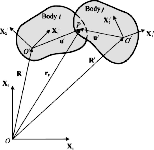
\includegraphics[height=7cm]{revolute.pdf}
\caption{Cerniera tra i corpi i e j}
\label{fig:2.1}
\end{figure}
In questo caso i corpi i e j hanno un solo grado di libertà relativo, ovvero la rotazione (si noti che siamo nel caso di moto piano).
In un sistema multibody le coordinate possono essere messe in relazione grazie ai vincoli, si potrà quindi scegliere quali coordinate sono dipendenti e quali indipendenti. 
Ogni equazione vincolare può eliminare una coordinata (che può essere quindi scritta in funzione di un'altra)
Perciò, un sistema di  $n$ coordinate ed $n_c$ equazioni vincolari ha $n-n_c$ coordinate indipendenti. 
Le coordinate indipendenti sono dette anche Gradi Di Libertà (GDL) del sistema.

\paragraph{Matrice Jacobiana $C_q$} Per poter considerare la presenza dei vincoli nella soluzione sarà necessario trovare relazioni tra i gradi di libertà dovuti ai vincoli, le quali andranno poi organizzate in un sistema di equazioni, per definire infine una matrice dei vincoli $C(q,t)$. \newline Le condizioni imposte da ciascun vincolo danno luogo ad un sistema di equazioni del tipo:
\begin{equation} \label{eq:Cqt}
C(q,t) = 0
\end{equation}
La relazione che definisce una cerniera nel caso di moto piano come mostrato in figura \ref{fig:2.1} ad esempio è data imponendo che la posizione del punto P considerato solidale al corpo i sia uguale alla posizione di P considerato solidale a j:
\[\overline{R}_i + A_i\overline{u}_i -\overline{R}_j - A_j\overline{u}_j = 0\]
Dove con R si indica la posizione assoluta delle origini dei riferimenti solidali ad i e j, con A la matrice di rotazione, con u la posizione di P e con i pedici i e j si indica che l'entità è relativa a quel corpo.
Ogni vincolo dà luogo ad numero di equazioni pari al suo grado di vincolo (ossia il numero di gradi di libertà bloccati dal vincolo). Poiché il sistema dovrà essere risolto numericamente con l'algoritmo di Newton-Raphson si rende necessario derivare rispetto agli spostamenti le equazioni dei vincoli ed organizzare i coefficienti in una matrice. La matrice così ottenuta sarà la matrice Jacobiana dei vincoli o sempicemente Jacobiano:
\begin{equation}
\label{eq:jacobian}
C_q =  \begin{bmatrix}
\frac{\partial C_1}{\partial q_1} & \frac{\partial C_1}{\partial q_2} & \qquad ... \qquad & \frac{\partial C_1}{\partial q_n} \\\
\frac{\partial C_2}{\partial q_1} & \frac{\partial C_2}{\partial q_2} & \qquad ... \qquad & \frac{\partial C_2}{\partial q_n} \\ . \\. \\ 
\frac{\partial C_{n_c}}{\partial q_1} & \frac{\partial C_{n_c}}{\partial q_2} & \qquad ... \qquad & \frac{\partial C_{n_c}}{\partial q_n}
\end{bmatrix} 
\end{equation}
Sviluppando l'equazione \ref{eq:Cqt} si può quindi scrivere:
\begin{equation} \label{jacobian_expansion}
C_q \delta q = 0
\end{equation}
Prendendo ad esempio il sistema con 2 soli corpi in figura [\ref{fig:2.1}] si ottiene:
\[ (C_1 , C_2)^T = \overline{R}_i + A_i\overline{u}_i -\overline{R}_j - A_j\overline{u}_j \]
Il sistema ha 6 coordinate e 2 equazioni vincolari date dall'unica cerniera. Le derivate rispetto alle posizioni sono banali, per quanto riguarda le rotazioni:
\[\frac{\partial C_1}{\partial \theta_i } = \frac{\partial A_i}{\partial \theta_i } \overline{u}_i  = A_i'\overline{u}_i\]
Dove A' indica la derivata della matrice di rotazione rispetto all'angolo che la definisce. Indicando un $u_{i,1}, u_{i,2}, u_{j,1} u_{j,2}$ le componenti nel primo e secondo asse dei vettori $u_i$ ed $u_j$, si può scrivere:
\begin{equation} C_q \delta q = 
\begin{bmatrix}
1 \quad & 0\quad & -u_{i,1}sin\theta_i-u_{i,2}cos\theta_i \quad& -1 \quad& 0 \quad& -u_{j,1}sin\theta_j-u_{j,2}cos\theta_j \\
0 \quad& 1 \quad& u_{i,1}cos\theta_i-u_{i,2}sin\theta_i \quad& 0 \quad& -1 \quad& u_{j,1}cos\theta_j-u_{j,2}sin\theta_j
\end{bmatrix}
\begin{pmatrix}
\delta R_{i,1} \\ \delta R_{i,2} \\ \delta \theta_i \\ \delta R_{j,1} \\ \delta R_{j,2} \\ \delta \theta_j 
\end{pmatrix} = 0
\end{equation}

\subsection{Moltiplicatori Lagrangiani}
Nella sezione  \ref{sec:Jabobian} è stato introdotto il calcolo dello Jacobiano e il concetto di coordinate dipendenti ed indipendenti. Per la soluzione numerica è conveniente considerare le reazioni vincolari come segue. \newline
\paragraph{Singolo Vincolo}
il jacobiano del vincolo $C_q$ tra i corpi \emph{i} e \emph{j} viene spezzato in 2 matrici:
\begin{equation} \label{eq:jacobian_composition}
C_q = \left[ C_{q^i} C_{q^j}\right]
\end{equation}
Si definisce quindi un sistema di forze \emph{equipollente} agente nelle origini dei sistemi di riferimento dei corpi di i e j. $\overline{\lambda}$ è il vettore delle forze e dei momenti esercitati dal vincolo:
\begin{equation} \label{eq:lambda}
\overline{\lambda} = - \begin{bmatrix} \overline{F} \\ \overline{M}
\end{bmatrix} \end{equation}
Le forze di reazione agenti sui corpi i e j sono:
\begin{equation}
\overline{F}^i = -\overline{\lambda} = 
\begin{bmatrix} \overline{F} \\ \overline{M} \end{bmatrix} \qquad ; 
\qquad \overline{F}^J = \overline{\lambda} = -\begin{bmatrix} \overline{F} \\ \overline{M} \end{bmatrix}
\end{equation}
Mentre, considerate nelle origini come sistema equipollente si ottiene:
\begin{equation}
Q^i_c = \begin{bmatrix} \overline{F} \\ \overline{M} + A^i\overline{u}^i_p x F \end{bmatrix} \qquad ; 
\end{equation}
Dove $\overline{u}^i_p$ è il vettore posizione di P (ove è applicato il vincolo) nelle coordinate di i e $A^i$ matrice di rotazione di i.
Da \cite{shabana94} si ha che:
\[A^i\overline{u}^i_p x F = {\overline{u}^i_p}^T {A_\theta^i}^T  \]
Si osserva quindi che le reazioni generalizzate possono essere espresse come:
\begin{equation}
\label{eq:lagrangemulti_to_reaction}
Q_c^i = -C^T_{q^i} \lambda
\end{equation}
\paragraph{Più vincoli}
Si può estendere la procedura illustrata al caso di più corpi collegati da più vincoli. Se sul corpo i ci sono $n_i$ vincoli le equazioni che li descrivono vengono espresse come:
\begin{equation} \label{eq:multiplejointeq} \begin{cases}
C_1(q,t) = 0 \\ C_2(q,t) = 0 \\ . \\ .\\ . \\ C_{n_i}(q,t) = 0
\end{cases}
\end{equation}
Ogni equazione vettoriale in \ref{eq:multiplejointeq} contiene tante equazioni quanti sono i \emph{gradi di vincolo} (gradi di libertà eliminati dal vincolo) del vincolo corrispondente. Dalla \ref{eq:lagrangemulti_to_reaction} si può estendere:
\begin{equation}\begin{cases}
Q_1^i = -\left( C_1 \right)^T_{q^i} \lambda_1 \\ Q_2^i = -\left( C_2 \right)^T_{q^i} \lambda_2 \\ . \\
Q_{ni}^i = -\left( C_{ni} \right)^T_{q^i} \lambda_{ni}
\end{cases} \end{equation}
Indicando con $Q^i_c$ la risultante delle reazioni vincolari sul corpo \emph{i} si può scrivere:
\begin{equation}\label{eq:reactions_result_body}
Q^i_c = -\left[ \left( C_1 \right)^T_{q^i} \quad \left( C_2 \right)^T_{q^i} \qquad \cdot\cdot\cdot 
\qquad \left( C_{ni} \right)^T_{q^i} \right] \begin{bmatrix}
\lambda_1 \\ \lambda2 \\ \cdot \\ \cdot \\ \cdot \\ \lambda_{n_i} 
\end{bmatrix} \end{equation}
Estendendo il calcolo a tutti gli $n_b$ corpi del sistema si calcolano le reazioni generalizzate dell'intero sistema $Q_c$. Essendo:
\[Q_c^i = -C^T_{q^i}\lambda\]
Si otterrà:
\begin{equation} \label{eq:sys_ge_reactions}
Q_c = \left[{Q_c^1}^T \qquad {Q_c^2}^T \quad \cdot \quad \cdot \quad \cdot {Q_c^{n_b}}^T\right]^T = \begin{bmatrix}Q_c^1 = -C^T_{q^1}\lambda \\ Q_c^2 = -C^T_{q^2}\lambda
\\ \cdot \\ \cdot \\ \cdot \\ Q_c^{n_b} = -C^T_{q^{n_b}}\lambda \end{bmatrix}
\end{equation}
Estendendo la composizione dello jacobiano in \ref{eq:jacobian_composition} si può quindi scrivere:
\begin{equation} \label{eq:reactions_result_sys}
Q_c = - \left[ C_{q^1} \qquad C_{q^2} \quad \cdot\quad\cdot\quad\cdot\quad Q_{q^{n_b}} \right]^T \lambda = -C_q^T\lambda
\end{equation}
\section{Equazioni della dinamica vincolata}
Per estendere quanto visto riguardo ai sistemi di particelle  nel cap. \ref{Formula di Lagrange} a sistemi di corpi rigidi sono necessarie alcune considerazioni:
\paragraph{Cinematica del corpo rigido}
La posizione di un corpo si esprime per mezzo di una traslazione dell'origine ed una rotazione:
\begin{equation} \label{eq:body_point_pos}
r^i = R^i + A^i\overline{u}^i
\end{equation}
Dove r è la posizione assoluta del punto P appartenente al corpo i, R è la posizione dell'origine del riferimento solidale ad i, A è la matrice di rotazione del corpo i e $\overline{u}$ è la posizione relativa di P. La velocità si ottiene derivando rispetto al tempo:
\begin{equation} \label{eq:body_point_vel}
\dot{r}^i = \dot{R}^i + \dot{A}^i\overline{u}^i = \dot{R}^i - A^i \tilde{\overline{u}}^i\overline{G}\dot{\theta}^i
\end{equation}
Con $\theta = \overline{q}$ quaternione unitario o vettore dei parametri di Eulero (indifferentemente), ed $\overline{G} = 2F(q^*)_-$ dell'equazione \ref{eq:1.9}. $\tilde{\overline{u}}$ è la matrice emisimmetrica ottenuta dalla posizione relativa $\overline{u}$ del generico punto P:
\begin{eqnarray} \tilde{\overline{u}}  = \begin{bmatrix}
0 & -x_3^i & x_2^i \\ x_3^i & 0 & -x_1^i \\ -x_2^i & x_1^i & 0 \end{bmatrix}\end{eqnarray}
Lo spostamento può essere dunque scritto in forma partizionata:
\begin{equation} \label{eq:body_point_vel_partform}
\dot{r}^i = \left[ I \qquad - A^i\tilde{\overline{u}}^i\overline{G}^i\right] \begin{bmatrix}\dot{R}^i \\ \dot{\theta}^i \end{bmatrix}  \end{equation}
\subsection{Matrice di massa}
Estendendo ad un corpo la definizione di energia cinetica data nell'equazione \ref{eq:part_kinenergy} si ottiene:
\begin{align} \label{eq:body_kinenergy}
T^i &= \frac{1}{2}\int_{V^i}\rho^i\dot{r}^{i^T} \dot{r}^idV^i 
\\ &= \frac{1}{2}\int_{V^i}\rho^i [\dot{R}^{i^T}\quad \dot{\theta}^{i^T}] \begin{bmatrix}I \\ - \overline{G}^{i^T}\tilde{\overline{u}^{i^T}A^{i^T}} \end{bmatrix} [I \quad -A^i\tilde{\overline{u}}^i\overline{G}^i] \begin{bmatrix} \dot{R}^i \\ \dot{\theta}^i \end{bmatrix}  dV^i \nonumber \\ &= \frac{1}{2}[\dot{R}^{i^T}\quad \dot{\theta}^{i^T}]\left\{\int_{V^i}\rho^i \begin{bmatrix}
I & -A^i\tilde{\overline{u}}^i\overline{G}^i \\ \quad sym_b \quad & \overline{G}^{i^T}\tilde{\overline{u}}^{i^T}\tilde{\overline{u}}^i\overline{G}^i
\end{bmatrix}  dV^i\right\} \begin{bmatrix} \dot{R}^i \\ \dot{\theta}^i \end{bmatrix} \nonumber
\\ &= \frac{1}{2}\dot{q}_r^{i^T}M^i\dot{q}_r^i
\end{align}
Con $sym_b$ si intende che il blocco è simmetrico.
$M^i$ è la \emph{matrice di massa} del corpo rigido i di volume $V^i$:
\begin{align}
M^i &= \int_{V^i}\rho^i \begin{bmatrix}
I & -A^i\tilde{\overline{u}}^i\overline{G}^i \\ \quad sym_b \quad & \overline{G}^{i^T}\tilde{\overline{u}}^{i^T}\tilde{\overline{u}}^i\overline{G}^i \end{bmatrix}  dV^i \\
&= \begin{bmatrix} m^i_{RR} & m^i_{R\theta} \\ \quad sym_b\quad &m^i_{\theta\theta}  \end{bmatrix} \end{align}
Si verifica facilmente che $M^i_{RR} = m^iI^{3x3}$ con $m_i$ massa dell'i-esimo corpo.
La matrice $M_{RR}$ associata alla traslazione del corpo è quindi una matrice diagonale costante.
La matrice associata all'interazione di rotazione e traslazione $m_{R\theta}$, ricordando che $a^i$ e $\overline{G}^i$ non dipendono dallo spazio si può esprimere come:
\begin{equation}
m^i_{R\theta} = - \int_{V^i}\rho^iA^i\tilde{\overline{u}}^i\overline{G}^idV^*i = -A^i \left[ \int_{V^i}\rho^i\tilde{\overline{u}}^i dV^i \right]  \overline{G}^i = -A^i\tilde{\overline{U}}^i\overline{G}^i
\end{equation}
Si noti che, qualora l'origine del riferimento coincida con il baricentro del corpo, $\tilde{\overline{U}}^i$ si annulla per la definizione di baricentro. 
Procedendo similmente per $m^i_{\theta\theta}$ si ottiene: \begin{align}
m^i_{\theta\theta} &= \overline{G}^{i^T}I_{\theta\theta}\overline{G}^i \\
I_{\theta\theta} &= \int_{V^i} \rho^i\tilde{\overline{u}}^{i^T} \tilde{\overline{u}}^i dV^i \\
I_{\theta\theta}&= \begin{bmatrix}i_{11} & i_{12} & i_{13} \\ \quad & i_{22} & i_{23} \\ sym & \quad & i_{33}\end{bmatrix}
\end{align}
Con $sym$ si nitende che la matrice è simmetrica
Con \begin{align} \label{eq:inertia_moment}
i_{jj} &= \int_{V^i} \rho^i[(x_k^i)^2+(x_l^i)^2]dV^i \qquad j\neq k\neq l\neq j ; \quad j,k,l = 1,2,3 \\
\label{eq:inertia_prod} i_{jk} &= \int_{V^i} \rho^ix_j^ix_k^i dV^i \qquad \qquad\qquad j\neq k \qquad j,k = 1,2,3
\end{align}
Gli elementi diagonali della matrice $I_{\theta\theta}$ descritti nell'equazione \ref{eq:inertia_moment} sono detti momenti d'inerzia, mentre i termini non diagonali di \ref{eq:inertia_prod} sono chiamati prodotti d'inerzia. Questi ultimi si annullano qualora il riferimento solidale al corpo sia \emph{principale di inerzia}.
L'energia cinetica di un corpo rigido può essere così scomposta:
\begin{align} \nonumber
T^i_{RR} &= \frac{1}{2}\dot{R}^{i^T}m^i_{RR}\dot{R}^i; \qquad T^i_{r\theta} = \dot{R}^{i^T}m^i_{r\theta}\dot{\theta}^i, \\ \nonumber
T^i_{\theta\theta} &= \frac{1}{2}\dot{\theta}^{i^T}m^i_{\theta\theta}\dot{\theta}^i =  \frac{1}{2} \overline{\omega}^{i^T}\overline{I}^i_{\theta\theta}\overline{\omega}^i
\end{align}
\subsection{Equazioni della dinamica dei corpi rigidi vincolati}
\paragraph{Equazioni della Dinamica}
L'equazione di Lagrange \ref{eq:lagrange_matrix} per i corpi rigidi assume la forma:
\begin{align} \label{eq:lagrange_body} \nonumber
\frac{d}{dt}\left( \frac{\partial T^i}{\partial\dot{q}}\right) -\frac{\partial T^i}{\partial q} -Q^i_e = 0 \\ \nonumber
\frac{d}{dt}\frac{\partial}{\partial \dot{q}}\left( \frac{1}{2}\dot{q}^{i^T}M^i\dot{q}^i \right) -\frac{\partial T^i}{\partial q} -Q^i_e = 0 \\ \nonumber
\frac{d}{dt}\left( M^i\dot{q}^i \right) -\frac{\partial T^i}{\partial q} -Q^i_e = 0 \\ 
 M^i\ddot{q}^i +\dot{M}^i\dot{q}^i -\frac{\partial T^i}{\partial q} -Q^i_e = 0 
\end{align}
Si consideri:
\begin{equation} \label{eq:Qv}
Q_v^i = -\dot{M}^i\dot{q}^i+\frac{\partial T}{\partial q}
\end{equation}
In verità l'espressione si riduce a \cite{shabana2005} : % pag 149 PDF 
\begin{align} \nonumber
Q_v^i = -\dot{M}^i\dot{q}^i+\left(\frac{\partial T}{\partial q}\right)^T =  [0_3^T \qquad -2\overline{\omega}^{i^T} \overline{I}^i_{\theta\theta}\dot{\overline{G}}^i ]
\end{align}
Infine, osservando che le equazioni sopra valgono per ogni corpo \emph{i} si ottiene in forma matriciale:
\begin{equation} \label{eq:dyn_sys_1stline}
M\ddot{q}+C_q^T\lambda = Q_e + Q_v
\end{equation}
con: 
\[M = \begin{bmatrix}
M^1 & \quad & \quad & \quad \\ \quad & M^2 & \quad & 0 \\ 0 & \quad & \ddots & \quad \\ \quad & \quad & \quad & M^{n_b}\end{bmatrix}\]
\[C_q^T = \begin{bmatrix} C^T_{q^1} \\ C^T_{q^2} \\ \vdots \\ C^T_{q^{n_b}} \end{bmatrix}; \qquad
Q_e = \begin{bmatrix} Q_e^1 \\\ Q_e^2 \\ \vdots \\ Q_e^{n_b} \end{bmatrix}; \qquad
Q_v = \begin{bmatrix} Q_v^1 \\\ Q_v^2 \\ \vdots \\ Q_v^{n_b} \end{bmatrix} \]
\textit{Si noti l'aggiunta di un termine vincolare e l'utilizzo del caso con coordinate indipendenti. Si veda il paragrafo seguente per approfondimenti.} \newline
Per considerare le equazioni di vincolo si deriva 2 volte rispetto al tempo l'equazione \ref{eq:Cqt} ottenendo:
\[C_q\ddot{q} + C_{tt} + (C_q\dot{q})_q\dot{q} + C_{qt}\dot{q}\]
Dove i pedici \emph{t} e \emph{q} indicano la derivazione parziale rispetto a tempo e posizione.
Considerando:
\begin{equation} \label{eq:Qd}
Q_d = - C_{tt} - (C_q\dot{q})_q\dot{q} - C_{qt}\dot{q}
\end{equation}
Da cui;
\begin{equation} \label{eq:dyn_sys_2ndline}
C_q\ddot{q} = Q_d
\end{equation}
Le equazioni \ref{eq:dyn_sys_1stline} e \ref{eq:dyn_sys_2ndline} danno luogo al seguente sistema:
\begin{equation} \label{eq:dyn_sys}
\begin{bmatrix} M & C_q^T \\ C_q & 0 \end{bmatrix}
\begin{bmatrix} \ddot{q}\\ \lambda \end{bmatrix} = 
\begin{bmatrix}
Q_e + Q_v \\ Q_d
\end{bmatrix}
\end{equation}
Questo sistema lineare può essere risolto per il vettore delle accelerazioni $\ddot{q}$ e dei moltiplicatori lagrangiani $\lambda$. A partire dalle condizioni iniziali è possibile integrare numericamente le accelerazioni per ottenere velocità e posizioni.
\paragraph{Formulazione Aumentata}
\textbf{Nota:} nella trattazione che porta all'equazione \ref{eq:dyn_sys_1stline} si è eliminato il termine $\delta q$ considerando le coordinate indipendenti. Nel caso di sistema vincolato tuttavia alcuni gradi di libertà saranno dipendenti a causa della presenza dei vincoli. La \emph{formulazione aumentata} \cite{shabana94} permette di trattare indipendentemente le coordinate di sistemi vincolati. \newline
Si considerino le equazioni \ref{eq:lagrange_body} e \ref{jacobian_expansion} ($Q_v$ si consideri compreso nel termine $Q_e$):
\begin{align} \nonumber \ \delta q^T\left[ M\ddot{q} - Q_e \right] = 0 \\ \nonumber
C_q \delta q = 0
\end{align}
Si deduce che  \[ \lambda^T C_q \delta q = 0 \] e quindi 
\[\delta q^T\left[ M\ddot{q} - Q_e +C_q^T\lambda \right] = 0 \]
Il vettore delle posizioni q viene partizionato in coordinate dipendenti ed indipendenti, e si ottiene:
\begin{equation}  [\delta q_i^T \quad \delta q_d^T] \left\{ \begin{bmatrix} M_{ii} & M_{id} \\ M_{di} & M_{dd}\end{bmatrix}
\begin{bmatrix}\ddot{q}_i \\ \ddot{q}_d \end{bmatrix}
- \begin{bmatrix} Q_{ei} \\ Q_{ed} \end{bmatrix}+ \begin{bmatrix}
C_{qi}^T \\ C_{qd}^T\end{bmatrix} \lambda
\right\}   = 0 \end{equation}
Ne consegue che:
\begin{align} \label{eq_aug_for_a}
\delta q_i^T \left[ M_{ii}\ddot{q}_i + M_{id}\ddot{q}_d - Q_{e_i} + C^T_{q_i}\lambda \right] = 0
\\ \label{eq_aug_for_b}
\delta q_d^T \left[ M_{di}\ddot{q}_i + M_{dd}\ddot{q}_d - Q_{e_d} + C^T_{q_d}\lambda \right] = 0
\end{align}
Le coordinate dipendenti possono sempre essere scelte in modo che $C_q$ sia non singolare in quanto le equazioni di vincolo sono linearmente indipendenti. Il vettore dei moltiplicatori lagrangiani sarà quindi la soluzione (unica) del sistema di equazioni \begin{equation}
C^T_{q_d} \lambda = Q_{e_d} - M_{id}\ddot{q}_i - M_{dd}\ddot{q}_d
\end{equation}
Ragion per cui i coefficienti di $\delta q$ nell' equazione \ref{eq_aug_for_b} sono tutti uguali a 0. Nell'equazione \ref{eq_aug_for_a} invece, poiché i $q_i$ sono indipendenti: \begin{equation}
M_{ii} \ddot{q}_i + M_{id}\ddot{q}_d +C^T_{q_i} \lambda = Q_{e_i}
\end{equation}
Combinando le 2 equazioni sopra si ottiene:
\[ \begin{bmatrix}  M_{ii} & M_{id} \\ M_{di} & M_{dd} \end{bmatrix}
\begin{bmatrix}\ddot{q}_i \\ \ddot{q}_d \end{bmatrix} +
\begin{bmatrix} C_{qi}^T \\ C_{qd}^T\end{bmatrix} \lambda = 
\begin{bmatrix} Q_{ei} \\ Q_{ed} \end{bmatrix}
\]
Da cui la forma generale: \begin{equation}
M\ddot{q} + C^T_q = Q_e	\end{equation}
Dando per noto il vettore delle forze esterne $Q_e$, le incognite sono $\ddot{q}$ e $\lambda$. Il numero di incognite è pari al numero di gradi di libertà indipendenti \emph{n} più il totale dei gradi di vincolo $n_c$. per questo viene aggiunta l'equazione \ref{eq:dyn_sys_2ndline}.
\part[Il Problema di Cauchy]
    {Il Problema di Cauchy\\[\bigskipamount] 
      \large Definizione e metodi numerici generici e specifici}
\chapter{Definizione e Proprietà dei metodi} \label{chap:cauchy}
\section{Definizione del problema di Cauchy}
Risolvere problemi di dinamica vincolata richiede di risolvere un sistema di equazioni differenziali-algebriche (DAE, \emph{Differential-Algebraic Equations}). La soluzione delle equazioni differenziali-algebriche passa per la soluzione delle equazioni differenziali ordinarie (ODE, \emph{Ordinary Differential Equation})
Il problema di Cauchy ai valori iniziali consiste un problema della forma:\newline
trovare $y(t)\in C^1(I)$ t.c. :
\begin{equation}  \label{eq:cauchy_def}  \begin{cases}
y'(t) = f(t, y(t)) \qquad  t\in I \\
y(t_0) = y_0 
\end{cases}
\end{equation}
La seconda equazione del sistema, ovvero il valore assunto dalla soluzione $y(t)$ in un dato istante $t_0$, è la condizione necessaria per l'unicità della soluzione, infatti Un’equazione differenziale ordinaria ammette in generale infinite soluzioni. Per fissarne una è necessario imporre una condizione che prescriva il valore assunto dalla soluzione in un punto dell'intervallo di integrazione.
La funzione \emph{f(t, y(t))} è assegnata e continua in entrambe le variabili nella striscia $ S = I \times (- \infty , + \infty)$. \newline
\textbf{Osservazione} se f continua in t, integrando \ref{eq:cauchy_def} si ottiene:
\begin{equation} \label{eq:cauchy_integral_equivalence}
y(t) - y_0 = \int^t_{t_0} y'(\tau)d\tau = \int^t_{t_0}f(\tau,y(\tau)) d\tau \end{equation}
L'equivalenza tra problema di Cauchy ed equazione integrala sarà sfruttata in seguito. \newline
\textbf{Nota:} in questa prima parte su tratteranno equazioni differenziali scalari, in seguito verrà esteso quanto riportato al caso di equazioni vettoriali.
%\paragraph{Esistenza ed unicità}
%\paragraph{Stabilità del problema}
\section{Metodi ad un passo} 
Nel seguito si introdurranno metodi numerici per la soluzione del problema di Cauchy. La simbologia utilizzata è la seguente: \begin{itemize}
    \item  $T \in \mathbb{R}_0^+ $ : Intervallo di integrazione da cui $ I = (t_0, t_0+T)$
    \item $h>0$ : ampiezza dei sottointervalli (detta \emph{passo di discretizzazione} o \emph{timestep})  
    \item $  t_n = t_0+nh; \quad n = 0,1,2... N_h$ la successione di nodi che discretizza I. Ovviamente $t_{N_h} \leq t_0+T$. \newline
\end{itemize}{}
\begin{definition} [Metodo single step] \label{def:single_step} 
Un metodo numerico per l'approssimazione del problema \ref{eq:cauchy_def}si definisce \emph{ad un passo} o \emph{single step} se $u_{n+1}$ dipende solo da $u_n$. In caso contrario si parla di metodi a più passi o \emph{multistep}.\end{definition}
\begin{definition} [Metodi impliciti ed espliciti]
Un metodo è detto \emph{esplicito} se $u_{n+1}$ non dipende da valori successivi a $t_n$. In caso contrario, ossia se $u_{n+1}$ dipende implicitamente da sé stesso tramite $f$ il metodo è \emph{implicito} \end{definition}
\paragraph{Metodo di Eulero in avanti (Eulero esplicito, Forward Euler)}
\begin{equation} \label{eq:Eul_Forw}
    u_{n+1} = u_n + h f_n
\end{equation}
\paragraph{Metodo di Eulero all'indietro (Eulero implicito, Backward Euler)}
\begin{equation}
    u_{n+1} = u_n + h f_{n+1}
\end{equation}
In entrambi i metodi di Eulero la derivata prima di $y$ con il rapporto incrementale ed entrambe la approssimazioni alle differenze finite di y sono accurate al primo ordine.
\paragraph{Metodo di Crank-Nicholson (del trapezio)}
\begin{equation}
    u_{n+1} = u_n + \frac{h}{2} \left[f_n+f_{n+1}\right]
\end{equation}
\paragraph{Metodo di Heun}
\begin{equation}
    u_{n+1} = u_n + \frac{h}{2} \left[f_n+f(t_{n+1},u_n,hf_n)\right]
\end{equation}

% \subsubsection{Metodi di Runge-Kutta}
% I metodi Runge-Kutta (RK) per aumentare l'accuratezza si avvalgono di molteplici valutazioni funzionali ad ogni passo. Questa strategia sacrifica la linearità e complica la valutazione dell'errore locale.
% In generale un metodo RK può essere scritto come 
% \begin{equation} \label{eq:RK_method_generalA}
%     u_{n+1} = u_n + hF(t_n, u_n, h; f), \qquad n\geq 0
% \end{equation}
% Dove $F$ è la \emph{funzione di incremento}:
% \begin{align} \label{eq:RK_method_generalB}
%     &F(t_n, u_n, h; f) = \sum_{i=1}^s b_i K_i \\  \label{eq:RK_method_generalC}
%     &K_i = f\left(t_n+c_i h, u_n + h \sum_{j=1}^s a_{ij}K_j\right), \qquad i = 1,2... s
% \end{align}
% In \ref{eq:RK_method_generalB} e \ref{eq:RK_method_generalC} \emph{s} indica il numero di stadi del metodo, mentre i coefficienti $\{a_{ij}\} \{c_i\} \{b_i\}$ definiscono completamente un metodo RK. 
% Per praticità è uso comune raccogliere i coefficienti nella \emph{matrice di Butcher}:
% \begin{equation}
% \begin{array}{c|cccc}
% c_1 & a_{11} & a_{12} & \hdots & a_{1s} \\
% c_2 & a_{21} & a_{22} & \hdots & a_{2s} \\
% \vdots & \vdots & \quad & \ddots & \vdots \\
% c_s & a_{s1} & a_{s2} & \hdots & a_{ss} \\  \hline
% \quad & b_1 & b_2 & \hdots & b_s \\
% \end{array}
% \end{equation}
% Appare evidente dalla \ref{eq:RK_method_generalC} che $K_i$ può essere calcolato esplicitamente solo se $a_{ij} = 0 \forall j \geq i$, e si parlerà in questo caso di \emph{schemi espliciti}. Alternativamente si parla di schemi \emph{impliciti e semi-impliciti} ma questi ultimi non verranno trattati.

\section{Metodi numerici e proprietà}

Nel seguito si indicherà con $u_j$ la soluzione approssimata nel nodo $t_j$ della soluzione esatta $y(t_j)$ o, brevemente, $y_j$. \newline
Allo stesso modo $f(t_j, u_j) = f_j$. Infine, poiché all'istante iniziale si dispone della soluzione esatta, $u_0 = y_0$.

Seconda lo definizione \ref{def:single_step} un metodo \textit{single step} può essere definito in generale come:
\begin{equation}\label{eq:Single_Step}
    u_{n+1} = u_n + \Phi(t_n , h, u_n , u_{n+1} ; f)
\end{equation}
la funzione $\Phi$ è detta \emph{funzione di incremento}, e definisce il valore assunto dall'approssimazione in $t_{n+1}$.
\paragraph{Errore di troncamento}
\begin{itemize}
\item Errore di troncamento locale: \newline

\begin{align} \label{eq:local_trunc_err} \nonumber
u_{n+1} &= u_n + h\Phi(t_n, u_n,f_n;h), \qquad 0\leq n \leq N_h - 1 , \qquad u_0 = y_0 \\
\nonumber y_{n+1} &= y_n + h\Phi(t_n, y_n,f_n;h) +\epsilon_{n+1} , \\ \Rightarrow
\epsilon_{n+1} &= h \tau_{n+1}(h) 
\end{align}
Dove $\epsilon_{+1}$ e $\tau_{n+1}$ sono il \emph{residuo} e l'\emph{errore di troncamento locale} nel nodo $t_{n+1}$.
\item Errore di troncamento globale \newline 
Si definisce \emph{errore di troncamento globale}  la quantità:
\begin{equation} \label{eq:glob_trunc_err}
\tau(h) = \underset{0 \leq n \leq N_{h-1}}{max} \left|\tau_{n+1}(h) \right|
\end{equation}
\end{itemize}
\paragraph{Consistenza}
Un metodo numerico ad un passo è completamente caratterizzato dalla funzione di incremento $\Phi$. Inoltre: 
\begin{equation} \label{eq:incr_limit}
\underset{h\rightarrow 0}{lim} (\Phi(t_n,y_nf(t_n,y_n);h)=f(t_n, y_n),\quad \forall t_n \geq t_0
\end{equation}
Da \ref{eq:incr_limit} e considerando che $y_{n+1}-y_n = hy'(t_n) + \mathcal{O}(h^2)$ si ha che
\begin{equation} \label{eq:consistenza}
\underset{h\rightarrow 0}{lim }(\tau(h)) = 0
\end{equation}
Questa proprietà esprime la consistenza del metodo numerico con il problema di Cauchy.

\paragraph{Zero stabilità}
Un metodo numerico è \emph{zero-stabile} se: \[\exists \quad
h_0, C, \epsilon_0 >0 \quad|\quad \forall h\in (0, h_0], \quad \epsilon \in (0, \epsilon_0], \quad 0\leq n \leq N_h \Rightarrow \] 
\begin{equation} \label{eq:zerostab} \left|z_n^{(h)}-u_n^{(h)} \right|\leq C\epsilon \end{equation}
Con \[\begin{cases}
z_{n+1}^{(h)}&=z_n^{(h)} + h\left[ \Phi (t_n, z_n^{(h)}, f(t_n, z_n^{(h)});h) + \delta_{n+1} \right] \quad n=0..N_{h-1}
\\ z_0^{(h)}&= y_0 + \delta_0 
\end{cases} \]\[ \begin{cases}
u_{n+1}^{(h)}&=u_n^{(h)} + h\Phi (t_n, u_n^{(h)}, f(t_n, u_n^{(h)});h) \quad n=0..N_{h-1}
\\ u_0^{(h)}&= y_0 + \delta_0  \end{cases} \]
La zero stabilità richiede che valga \ref{eq:zerostab} in un intervallo limitato $\forall h\leq h_0$. Questa proprietà è relativa al metodo, non al problema. 
\begin{theorem}[Zero Stabilità] \label{teo:zerostab}
Si consideri un metodo numerico ad un passo per la soluzione del problema di Cauchy. Se la funzione di incremento $\Phi(t_n, u_n,f_n;h)$ è lipschitziana di costante $\Lambda$ rispetto al secondo argomento, uniformemente rispetto ad h e a $t_j \in [t_o, t_0 +T]$ allora il metodo è zero-stabile.  \cite{Quarteroni} \end{theorem}
\paragraph{Convergenza}
Un metodo è \emph{convergente} se: \begin{equation} \label{eq:def_convergenza}
\forall \quad n = 0,1,2....,N_h \qquad \left| u_n - y_n \right| \leq C(h)\end{equation}
$C(h)$ è un infinitesimo di $h$. 
Il metodo di dice \emph{convergente di ordine p} se $C(h) = \mathcal{O}(h^p)$ cioè se $\exists C>0 t.c. C(h) \leq Ch^p \forall h>0$ con $p$ massimo.
\begin{theorem}[Convergenza] \label{teo:converg}
Nelle ipotesi del teorema \ref{teo:zerostab}, per il lemma di Gronwall: \begin{equation}
\left|y_n - u_n\right| \leq \left(\left|y_0-u_0\right| + nh\tau(h)\right)e^{nh\tau}, \qquad 1\leq n\leq 
N_h \end{equation} 
Se vale l'ipotesi di consistenza \ref{eq:consistenza} ed $|y_0-u_0| \rightarrow 0$ per $h\rightarrow 0$ il metodo è convergente.Se $|y_0-u_0| = \mathcal{0}(h^p)$ ed il metodo ha ordine p, allora converge con ordine p \end{theorem}
\textbf{Lemma di Gronwall} \newline
Siano $k_n, \phi_n$ successioni (la prima non-negativa) tali che: \begin{equation}\begin{dcases}
\phi_0 \leq g_0 \\ \phi_n \leq g_0 + \sum_{s=0}^{n-1}p_s + \sum_{s=0}^{n-1}k_s\phi_s \qquad n\geq 1
\end{dcases} \end{equation}
Se $g_0, p_n \geq 0 \forall n \geq 0$ allora:
\begin{equation}
\phi_n \leq \left( g_0 + \sum_{s=0}^{n-1}p_s  \right)
exp \left(\sum_{s=0}^{n-1}k_s \right)
\end{equation}
Si osserva quindi che un metodo (single step) consistente e zero-stabile è necessariamente convergente. Questa proprietà è chiamata \emph{teorema di Lax-Richtmyer o di equivalenza} ed è di estrema rilevanza nell'analisi numerica.


\paragraph{Assoluta stabilità}
L'assoluta stabilità è una proprietà che riguarda il comportamento asintotico del metodo. Un metodo si dice assolutamente stabile se, con $h$ fissato, $u_n$ è limitata per $t_n\rightarrow +\infty$.

Si definisce un \emph{problema modello}
\begin{equation}\label{eq:model_cauchyprob}
    \begin{cases} y'(t) = \lambda y(t) \qquad t>0 \\ y(0) = 1 \end{cases} \end{equation}
La soluzione di \ref{eq:model_cauchyprob} è $y = e^{ \lambda t}$, inoltre se $\mathcal{R}(\lambda)<0$, $u_n\rightarrow 0$
% \subsubsection{Proprietà dei metodi di Runge-Kutta}
% \paragraph{Consistenza}
% Si definisce l'errore di troncamento locale a partire dalla formula del residuo:
% \begin{equation}
%     h \tau_{n+1}(h) = y_{n+1} - y_n -hF(t_n, y_n, h; f)
% \end{equation}
% Si verifica che il metodo è consistente, ossia $\tau(h) = max_n|\tau_n(h)| \rightarrow 0$ per $h\rightarrow 0$, se e solo se:
% \begin{equation}
%     \sum_{i=1}^s b_i = 1
% \end{equation}
% \paragraph{Convergenza}
% Trattandosi di un metodo single step, per il teorema \ref{teo:converg} la consistenza implica la convergenza, pertanto avrà le medesime condizioni.

\subsection{Proprietà dei metodi}
\begin{definition} [Assoluta Stabilità]
Un metodo è assolutamente stabile se l'approssimazione della soluzione di \ref{eq:model_cauchyprob}
\begin{equation} \label{eq:abs_stab}
    |u_n| \rightarrow 0 \qquad \text{per} \qquad t_n \rightarrow +\infty
\end{equation}
\end{definition}

Si definisce \emph{problema di Cauchy lineare} o \emph{problema modello}
\begin{equation}  \label{eq:cauchy_def}  \begin{cases}
y'(t) = \lambda y(t) \qquad  t > 0 \\
y(t_0) = 1 
\end{cases}
\end{equation}

Dq questa definizione si può inoltre definire \emph{regione di assoluta stabilità} del metodo il sottoinsieme di $\mathbb{C}$ 
\begin{equation}
    \mathbb{A} = \{ z=h\lambda \in \mathbb{C} \qquad \text{t.c. \ref{eq:abs_stab} è soddisfatta} \}
\end{equation}
\begin{definition}[Metodi A-stabili e condizionatamente stabili]
Un metodo è detto \emph{A-stabile} se $\mathcal{A} \cap \mathbb{C}^- = \mathbb{C}^-$ ovvero se \ref{eq:abs_stab} è soddisfatta $\forall\lambda\in \mathbb{C}^-$ incondizionatamente rispetto ad $h$, mentre qualora siano richiesta condizioni su h sono condizionatamente stabili. 
I metodi $\theta$ stabili, invece, sono metodi Multistep per i quali A contiene la regione angolare definita dagli $z \in \mathcal{C}$ tali che $-\theta < \pi - arg(z) < \theta$ con $\theta \in  (0, \pi/2)$.
\end{definition}
\begin{theorem}[Prima Barriera di Dahlquist]
Non esistono metodi multistep lineari zero-stabili a q-passi con ordine maggiore di q + 1 se q è dispari, q + 2 se q è pari.
\end{theorem}
\begin{theorem}[Seconda Barriera di Dahlquist]\label{theo:DahlquistII}
Un metodo multistep lineare esplicito non può essere né A-stabile, né $\theta$-stabile. Inoltre, non esistono metodi multistep lineari A-stabili di ordine superiore a due. Per ogni
$\theta \in (0, \pi/2)$ esiste almeno un metodo multistep lineare $\theta$-stabile a q passi di
ordine q solo per q = 3 e q = 4.
\end{theorem}
Le barriere di Dahlquist limitano allo stesso modo i metodi ad un passo, considerabili come casi di metodi multistep con $n=1$.


\section{Sistemi di equazioni}
Il sistema di ODE del primo ordine:
\begin{equation}
 \avect{y}' = \amatr{F}(t, \avect{y})
\end{equation}
Con $\avect{y}\in \mathbb{R}^n$ vettore soluzione e $\amatr{F}:\mathbb{R} \times \mathbb{R}^n \rightarrow \mathbb{R}^n$. La soluzione dipende sempre dal valore iniziale che in questo caso è un vettore di $n$ elementi $\avect{y}_0 \in \mathbb{R}^n$.
\paragraph{Lipschitzianità ed esistenza della soluzione}
Se $\amatr{F} è Lipschitziana $ ossia se , essendo continua su $D = [t_0,T]\times \mathbb{R}^n$, con $t_o, T$ finiti esiste $L$ tale che:
\begin{equation}
    \norm{\amatr{F}(t,\avect{y}) - \amatr{F}(t,\overline{\avect{y}})} \leq L \norm{\avect{y}- \overline{\avect{y}}}
\end{equation}
per ogni $(t, \avect{y}), (t, \overline{\avect{y}}) \in D$; si dimostra che esiste ed è unica la soluzione $\avect{y}$  continua in $D$ del problema \ref{eq:cauchy_def}.


Per quanto riguarda le soluzioni numeriche del detto problema i metodi visti (e quelli riportati in seguito) sono estendibili al caso di sistemi di equazioni. 
\chapter{Metodi numerici specifici}
Verranno di seguito illustrati metodi numerici per la soluzione del problema di Cauchy espressamente ideati per l'applicazione a simulazioni multibody.

Dal momento che d'ora in avanti si farà specifico riferimento alla dinamica di sistemi meccanici si riprenderà la notazione utilizzata nella parte \ref{part:LagrDyn}. In luogo dei vettori $\avect{y}$ ed $\avect{y}'$ si avranno $\{\avect{q} , \avect{v}\}$ e $\{\avect{v} , \avect{a}\}$; rispettivamente posizioni e velocità e velocità ed accelerazioni del sistema. Sempre riprendendo la notazione si avrà \begin{itemize}
    \item $\amatr{C} = \amatr{C}(\avect{q},t)$ vettore delle equazioni vincolari
    \item $\amatr{C_q} =\frac{\partial\avect{C}}{\partial q}$
    \item $\amatr{M}$ matrice di massa
    \item $\avect{\lambda}$ vettore di moltiplicatori lagrangiani (reazioni vincolari)
    \item $\avect{f}$ forze agenti sul sistema
    \item $l$ indica lo step di integrazione
    \item Con $h \in \mathbb{R}$ si indica sempre l'ampiezza del \emph{timestep}. 

\end{itemize}

Riguardo le equazioni della dinamica dei sistemi verranno utilizzate la prima equazione della formulazione lagrangiana \ref{eq:dyn_sys_1stline} e l'equazione delle condizioni di vincolo \ref{eq:Cqt}. Dato lo stato del sistema è possibile trovare accelerazioni e reazioni vincolari grazie a queste relazioni.
A proposito dell'equazione della dinamica dei sistemi vincolati \ref{eq:dyn_sys_1stline} essa può essere riscritta come: \[\amatr{M}\avect{a} + \amatr{C}_q^T\avect{\lambda} = \avect{f} \] Dove il vettore delle forze applicate $f$ comprende sia le forze esterne $Q_e$ che il termine cosiddetto giroscopico $Q_v$. Si consideri inoltre che, a seconda della letteratura di riferimento, l'equazione \ref{eq:lambda} che definisce $\lambda$ può avere o no il segno meno. Nella implementazione seguente si è scelta la seconda opzione, ragion per cui si scriverà d'ora in avanti:
\begin{equation}\label{eq:dynamics}
    \amatr{M}\avect{a}-\amatr{C}_q^T\avect{\lambda}-\avect{f} = 0
\end{equation}

Inoltre nel corso del capitolo verrà menzionato un fenomeno chiamato smorzamento numerico (\textit{numerical damping}), un errore numerico che si manifesta come la presenza di uno smorzamento fittizio. Si fornisce una trattazione più dettagliata del fenomeno in sez. \ref{sec_numdamp}.
 \section{Newmark Method}
 Questo metodo nasce per studiare la risposta dinamica di strutture e solidi modellati con gli elementi finiti e per questa ragione è assai diffuso nella comunità FEM. %La formulazione si basa sul Teorema di Lagrange, ovvero sull'esistenza di un $\avect{a}_{\beta}\quad t.c. \quad \avect{v}^{l+1} = \avect{v}^l h\avect{a}_{\beta}$ con $\avect{a}^l \leq \avect{a}_{\beta} \leq\avect{a}^{l+1}$
 
 \begin{align} \label{eq:NewmarkDef}
 \amatr{M}\avect{a}^{l+1}-(\amatr{C}_q^t\avect{\lambda}+\avect{f})^{l+1}&=0 \\
 \avect{v}^{l+1}- \avect{v}^l -h \left[(1-\gamma)\avect{a}^l+\gamma \avect{a}^{l+1}\right]&=0 \\
\avect{q}^{l+1}-\avect{q}^l - h \avect{v}^l-\frac{h^2}{2}\left[(1-2\beta)\avect{a}^l+2\beta\avect{a}^{l+1}\right]&=0
 \end{align}
 %È un metodo del second'ordine, implicito ed incondizionatamente stabile per determinati valori dei coefficienti che lo caratterizzano. 
 Caratteristiche del metodo \cite{newmark59}:
\begin{itemize}
    \item si basa sul Teorema di Lagrange, ovvero sull'esistenza di un $\avect{a}_{\beta}\quad $tale che $ \quad \avect{v}^{l+1} = \avect{v}^l + h\avect{a}_{\beta}$ con $\avect{a}^l \leq \avect{a}_{\beta} \leq\avect{a}^{l+1}$
    \item $\gamma$ è normalmente compreso tra 1/2 ed 1
    \item $\gamma$ è solitamente posto uguale ad 1/2, unico valore per il quale si ottiene ordine di convergenza quadratico. 
    \item $\beta$ è compreso tra 0 ed 1.
    \item per $\beta =1/4, \gamma= 1/2$ si ha il metodo dell'accelerazione costante.
    \item per $\beta =1/6, \gamma= 1/2$ si ha il metodo dell'accelerazione lineare.
    \item Per $\gamma \geq 1/2$ e $\beta \geq  \frac{(\gamma + \frac{1}{2})^2}{4}$ il metodo è incondizionatamente stabile.
    \item Il metodo dell'accelerazione costante è incondizionatamente stabile.
    \item Lo smorzamento numerico è nullo per $\gamma = \frac{1}{2}$ mentre si manifesta per valori maggiori, crescendo  con $\gamma$

\end{itemize}
 \section{HHT Method}
 Il metodo Hilber-Hughes-Taylor è una generalizzazione del metodo di Newmark che aggiunge un ulteriore parametro $\alpha$ \cite{Negrut2006}. 
 \begin{align}
\amatr{M}\avect{a}^{l+1}-(1+\alpha)(\amatr{C}_q^t\avect{\lambda}+\avect{f})^{l+1}+\alpha(\amatr{C}_q^T\avect{\lambda}+f)^l&=0 \\
\avect{v}^{l+1}-\avect{v}^l-h[(1-\gamma)\avect{a}^l+\gamma\avect{a}^{l+1}] &=0 \\
\avect{q}^{l+1}-\avect{q}^l-h\avect{v}^l-\frac{h^2}{2}[(1-2\beta)\avect{a}^l+2\beta\avect{a}^{l+1}] &=0
 \end{align}
 Caratteristiche del metodo \cite{Hilber1977} \cite{Hughes1983}:
\begin{itemize}
    \item Il parametro $\alpha$ permette di controllare la dissipazione numerica. Per $\alpha = 0$ il metodo coincide con Newmark, al decrescere del parametro vengono smorzate le frequenze più alte.
    \item Basandosi sull'esperienza la letteratura suggerisce di porre $0\leq \alpha \leq1/3$ , $\beta = (1-\alpha)^2/4 $ e $\gamma = 1/2 - \alpha$.  
    \item A-stabile (per i valori dei parametri riportati sopra)
    \item Ordine di convergenza 2 (per i valori dei parametri riportati sopra)
\end{itemize}
\section{Generalized-$\alpha$ Method}
\paragraph{Confronto fra i metodi in termini di convergenza e stabilità}
Dalla seconda barriera di Dahlquist (Teorema \ref{theo:DahlquistII}) sappiamo che non esistono metodi multistep lineari A-stabili di ordine superiore a due. Il metodo dei trapezi utilizzato per DAE (\emph{Differetial-Algebraic Equations}) dà luogo a reazioni vincolari oscillanti instabili se utilizzato per sistemi vincolati. Al contrario i metodi HHT e generalized-$\alpha$, introdotto nel seguito, sono tra i pochi integratori di ordine 2 che possono risolvere DAE vincolate.

Il metodo generalized-$\alpha$ \cite{generalizedAlphaHulbert93} \cite{JayNegrut2008} è un'evoluzione del metodo HHT, nel quale tutti i parametri vengono settati a partire da un solo parametro $\rho_\infty$. È un metodo del second'ordine come accennato in precedenza, e permette il controllo della dissipazione numerica.

Si definisce come segue:
 
\begin{align} \label{eq:Gen-Alpha1}
\amatr{M}\avect{a_*}^{l+1}-(\amatr{C}_q^t\avect{\lambda}+f)^{l+1}&=0 \\ \label{eq:Gen-Alpha2}
(1-\alpha_m)\avect{a}^{l+1}+\alpha_m\avect{a}^l = (1-\alpha_f)\avect{a_*}^{l+1} + \alpha_f\avect{a_*}^l&=0 \\
\avect{v}^{l+1}-\avect{v}^l-h[(1-\gamma)\avect{a}^l+\gamma\avect{a}^{l+1}] &=0 \\
\avect{q}^{l+1}-\avect{q}^l-h\avect{v}^l-\frac{h}{2}[(1-2\beta)\avect{a}^l+2\beta\avect{a}^{l+1}] &=0
\end{align}

Come anticipato tutti i parametri elencati vengono settati a partire da un unico parametro $\rho_\infty \in [0,1]$:
\begin{align}
    \alpha_m &= \frac{2\rho_\infty-1}{1+\rho_\infty} \\
    \alpha_f &= \frac{\rho_\infty}{1+\rho_\infty}   \\
    \beta &= \frac{1}{4}\left(\gamma+\frac{1}{2} \right)^2 \\
    \gamma &= \frac{1}{2}+\alpha_f - \alpha_m
\end{align}

Si noti che: \begin{itemize}
    \item Per $\rho_\infty=0$ si ha massima dissipazione asintotica ed il metodo ha smorzamento massimo.
    \item Il metodo HHT è come il metodo generalized-$\alpha$ con $\alpha_m =0$ e $\alpha_f = \alpha$. Effettivamente i metodi hanno proprietà simili. Per verificarlo si sostituisca $\avect{a_*}$ calcolato in $l$ ed $l+1$ secondo
    \ref{eq:Gen-Alpha1} in  \ref{eq:Gen-Alpha2} ($\amatr{M}$ è sempre invertibile).
    \item Per $\rho_\infty=1$ d'altra parte non c'è dissipazione numerica, come nel metodo dei trapezi. A differenza di questo, tuttavia, il metodo generalized-$\alpha$ si comporta bene in presenza di vincoli. 
\end{itemize}
Nella pratica uno smorzamento numerico è quasi sempre inserito anche se il sistema fisico non è dissipativo, onde evitare divergenze in simulazioni prolungate. Di solito si utilizza un valore intermedio di $\rho_\infty$, che aiuta a scartare frequenze di oscillazione elevate di scarso interesse. Solitamente il valore di $\rho_\infty$ viene trovato euristicamente, partendo da valori prossimi a 0 ed aumentandolo gradualmente fino alla comparsa di armoniche a frequenza elevata.

\chapter{Applicazione dei metodi alle simulazioni multibody}
In questo capitolo si vedrà come applicare i metodi numerici visti nel capitolo \ref{chap:cauchy} alle simulazioni multibody.

Si noti che nella definizione del problema di Cauchy (eq. \ref{eq:cauchy_def}) la funzione $f(t, y(t))$ viene considerata assegnata. Questo non accade in una simulazione, dal momento che lo stato del sistema non è noto a priori. \newline
Si consideri il sistema \ref{eq:dyn_sys}: la matrice dei coefficienti ed il vettore dei termini noti dipendono dallo stato futuro, e non è pertanto possibile calcolare direttamente $\avect{\Ddot{q}}$ e $\avect{\lambda}$ nel timestep futuro $t+1$ come richiesto dai metodi impliciti. \newline A questi algoritmi andrà pertanto abbinato il metodo di Newton per i sistemi.


\section{Cenni al metodo di Newton-Raphson o Metodo delle Tangenti}
\subsection{Metodo di Newton per la soluzione di equazioni non lineari}
Il metodo di Newton \cite{Quarteroni} può essere utilizzato per approssimare numericamente gli zeri di una funzione di una variabile reale, ossia data \(f:\mathbb{R} \rightarrow \mathbb{R}\) si cerca $\alpha\in \mathbb{C}\quad t.c.\quad f(\alpha)=0 $ \newline
Se $f \in C^1([a,b])\quad con \quad [a,b]\subset\mathbb{R} \quad t.c. \quad f(a)f(b) < 0 \quad e \quad f'(x) \neq 0 \forall x \in [a,b]$ si può procedere iterativamente al calcolo della radice una volta assegnato il valore iniziale $x^{0}$:
\begin{equation} \label{eq:Newton_1d}
    x^{(k+1)} = x^{(k)} - \frac{f\left(x^{(k)}\right)}{f'\left(x^{(k)}\right)}
\end{equation}
Sebbene il metodo richieda 2 valutazioni funzionali controbilancia l'onere computazionale con un ordine di convergenza 2 (quando la radice è semplice).
\begin{figure}[h!]
\centering
\includegraphics[height=8cm]{newtonRaphsonMethod.png}
\caption{Rappresentazione grafica per i passi del metodo di Newton}
 \label{fig:Newton_1d}
\end{figure}
\subsection{Metodo di Newton per la soluzione di sistemi}
Il metodo di Newton può essere esteso al caso di sistemi di equazioni. 
Il metodo può essere esteso al caso di sistemi di equazioni. Indicando con l'apice n l' n-esimo passaggio, con $\amatr{F}$ il sistema di equazioni e con $\amatr{J}$ il jacobiano di quest'ultimo si procede dato $\avect{x}{(0)}$ come segue:
\begin{align} \label{eq:NewtonRaphsonA}
    \amatr{J}\left( \avect{x}^{(n)} \right) \avect{\delta x}^{(n)} = - \amatr{F}\left( \avect{x}^{(n)} \right) \\
    \label{eq:NewtonRaphsonB}  \avect{x}^{(n+1)} = \avect{x}^{(n)} + \avect{\delta x}^{(n)} 
\end{align}
L'onere computazionale di questo metodo consiste nel risolvere ad ogni passaggio un sistema lineare di matrice $\amatr{J}$.

\section{Smorzamento Numerico} \label{sec_numdamp}
Lo smorzamento numerico (\textit{numerical damping}) indica un errore numerico, che si manifesta come la comparsa di uno smorzamento fittizio, tipica dei metodi impliciti ed, in taluni casi, semi-impliciti. Questo fenomeno è ben osservabile in un sistema massa-molla senza smorzatore, le cui oscillazioni dovrebbero mantenersi ad ampiezza costante, mentre diminuiscono nel tempo. Questo fenomeno si accentua al diradarsi del \textit{timestep}.
\subsection{Esempio numerico: smorzamento numerico in un sistema massa-molla implementato in Matlab}
Per osservare quanto affermato si riporta un esempio numerico del sistema massa molla. Con la solita notazione possiamo scrivere :\[\begin{cases}\frac{v^{l+1}-v^l}{h}M = f^{l+1}\\ q^{l+1}= q^l+v^{l+1}h \end{cases}\]
Nel caso del sistema massa-molla si avrà : \[f^l = Mg-Kq^l \]O, in presenza di smorzatore \[ f^l = Mg-Kq^l-Cv^l\]
Da cui:  \[ \left(v^{l+1}-v^l\right)M = h\left(  Mg-Kq^{l+1} -Cv^{l+1} \right)  \]
Sostituendo il valore di $q^{+1}$ si ottiene:
\[ \left(v^{l+1}-v^l\right)M = h\left(  Mg-K(q^l+v^{l+1}h) -Cv^{l+1} \right)  \]
Si può quindi scrivere:
\[ v^{l+1}\left(M+Kh^2+Ch\right) = Mv^l + h\left(  Mg-Kq^l \right)  \]
Possiamo quindi esprimere $v^{l+1}$
\[ v^{l+1} = \frac{ Mv^l + Mgh -Khq^l }{\left(M+Kh^2+Ch\right)}  \]
A questo punto si procede ad implementare in Matlab un algoritmo che risolve numericamente il sistema con \textit{timestep} crescente così da poter osservare l'andamento della smorzamento numerico. Si riporta la porzione di codice più significativa, ovvero il ciclo \textit{while} che calcola velocità e posizione nell'istante successivo e le memorizza.


\noindent\rule{\textwidth}{1pt}\newline  $ 
    while \  t<= Tmax \\
        vl1 = (m*v+m*g*dt-k*x*dt)/(m+k*dt^2+c*dt); \\
        xl1 = x + dt*vl1; \\
        t = t+ dt; \\
        v = vl1; \\
        x = xl1; \\
        j = j+1; \\
        v_{vett}(j) = vl1; \\
        x_{vett}(j) = xl1; \\
        t_{vett}(j) = t; \\
    end$ \newline
\noindent\rule{\textwidth}{1pt}
Di seguito sono riportati i grafici di spostamento e velocità della simulazione del sistema massa-molla che utilizza il loop riportato. Sebbene sia presente un termine di smorzamento esso è in realtà nullo. 

\begin{figure}[ht]
\centering
\includegraphics[height=5cm]{Figure/position.pdf}
\caption{Posizione della massa nel sistema massa-molla in funzione del tempo al variare del timestep}
 \label{fig:Newton_1d}
\end{figure}

\begin{figure}[h!]
\centering
\includegraphics[height=5cm]{Figure/speed.pdf}
\caption{Velocità della massa nel sistema massa-molla in funzione del tempo al variare del timestep}
 \label{fig:Newton_1d}
\end{figure}

Ciononostante si nota una progressiva diminuzione dell'ampiezza delle oscillazioni, più accentuata all'aumentare del \textit{timestep}, mentre in condizioni di smorzamento nullo la soluzione analitica prevederebbe oscillazioni ad ampiezza costante. 

Lo smorzamento fittizio (in quanto derivato da un errore numerico e senza alcun riscontro fisico) osservabile è la manifestazione dello smorzamento numerico in questione. Infatti l'unica differenza tra le soluzioni è il progressivo aumento del \textit{timestep}.


\section{Algoritmi di soluzione per metodi impliciti}
\paragraph{Eulero implicito}
Di seguito si illustra l'applicazione del metodo di integrazione di Eulero implicito (Backward Euler) ad un sistema multibody in presenza di vicoli.
Si riprende l'equazione \ref{eq:dyn_sys}. Come accennato in precedenza non è possibile conoscere direttamente il valore delle forze nello stato $l+1$. Per pervenire ad una soluzione è necessario includere l'integrazione numerica all'interno di un'iterazione di Newton-Raphson.

Per un sistema multibody il metodo di Eulero implicito può essere scritto come il seguente sistema che chiameremo \textbf{G}
\begin{align} \label{eq:eulforw_Gq}
    \avect{q}^{l+1}-\avect{q}^l - \avect{v}^{l+1}h &= 0 \\ \label{eq:eulforw_Gv}
    \amatr{M}(\avect{v}^{l+1} -\avect{v}) - h\avect{f}^{l+1} - h\amatr{C}_q^T \avect{\lambda}^{l+1} &= 0 \\ \label{eq:eulforw_Glam}
    \amatr{C}(\avect{q}^{l+1} , t^{l+1}) &= 0
\end{align}
Per procedere alla soluzione iterativa con Newton come anticipato si deve esprimere lo Jacobiano del sistema \textbf{G}:
\begin{equation} \label{eq:eulforwjacob} \amatr{J} =
    \begin{bmatrix} I & -hI   & 0 \\
    -h\nabla_q\avect{f}^{l+1} & \amatr{M}-h\nabla_v\avect{f}^{l+1} &  -h\amatr{C}_q^T \\
    \amatr{C}_q               &  0                                 &    0  \end{bmatrix}
\end{equation}
Utilizzando il procedimento illustrato in \ref{eq:NewtonRaphsonA} si scrive:
\begin{equation} \label{eq:eulforw_iterstep}
    \amatr{J} \left\{\begin{array}{c}\Delta\avect{q}^{l+1} \\ \Delta\avect{v}^{l+1} 
    \\ \Delta\avect{\lambda}^{l+1} \end{array} \right\} = -\amatr{G} \end{equation}
Dalla prima riga dell'equazione \ref{eq:eulforw_iterstep}:
\[ \Delta\avect{q}^{l+1} = h\Delta\avect{v}^{l+1} -\avect{q}^{+1} +\avect{q}^l + h\avect{v}^{l+1} \]
E, differenziando l'equazione \ref{eq:eulforw_Gq} si ottiene 
\begin{equation}
    \Delta \avect{q}^{l+1} = h \Delta \avect{v}^{l+1}
\end{equation}

Questa approssimazione è vera solo in prossimità della soluzione ma viene comunemente usata per evitare la complicazione che proviene dal considerare tutti i termini del sistema.
Grazie a questa relazione possiamo eliminare la dipendenza di $\avect{q}^{l+1}$ da $\Delta \avect{q}^{l+1}$, infatti la prima equazione di \ref{eq:eulforw_iterstep} si semplifica divenendo identica alla \ref{eq:eulforw_Gq} e il sistema \ref{eq:eulforw_iterstep} diventa: 

\begin{equation}
        \begin{bmatrix} I & -hI   & 0 \\
    -h\nabla_q\avect{f}^{l+1} & \amatr{M}-h\nabla_v\avect{f}^{l+1} &  -h\amatr{C}_q^T \\
    \amatr{C}_q               &  0                                 &    0  \end{bmatrix}
    \left\{\begin{array}{c}h\Delta\avect{v}^{l+1} \\ \Delta\avect{v}^{l+1} 
    \\ \Delta\avect{\lambda}^{l+1} \end{array} \right\}
    = -\amatr{G}
\end{equation}
La seconda e terza equazione possono essere riscritte come segue, la prima è riportata in fondo e vengono aggiunti i passaggi del procedimento di Newton Raphson \ref{eq:NewtonRaphsonB} per $v$ d $\lambda$.
\[
    \begin{bmatrix}\left[ M-h^2\nabla_q\avect{f}^{l+1}-h\nabla_v\avect{f}^{l+1} \right] & \amatr{C}_q^T \\\amatr{C}_q &0 \end{bmatrix} \left\{\begin{array}{c} \Delta\avect{v}^{l+1}  \\ 
    -h\Delta\avect{\lambda}^{l+1} \end{array} \right\} = \] \begin{equation} \label{eq:eulfor_NRiter1} =
    \left\{\begin{array}{c} (\avect{v}^l-\avect{v}^{l+1})\amatr{M}+h\avect{f}^{l+1}+h\amatr{C}_q^T \avect{\lambda}^{l+1}\\ -\frac{\amatr{C^{l+1}}}{h} \end{array} \right\}
\end{equation}
\begin{equation}
        \avect{v}_{n+1}^{l+1} = \avect{v}_n^{l+1} + \Delta\avect{v}^{l+1}
\end{equation}
\begin{equation}
        \avect{\lambda}_{n+1}^{l+1} = \avect{\lambda}_n^{l+1} + \Delta\avect{\lambda}^{l+1}
\end{equation}
\begin{equation} \label{eq:eulfor_NRiter4}
        \avect{q}^{l+1} = \avect{q}^l + h\avect{v}_{n+1}^{l+1}
\end{equation}
Si noti che \begin{itemize}
    \item L'indice dell'iterazione è passato al pedice in quanto l'apice è già utilizzato per indicare il timestep.
    \item $\avect{q}$ non dipende da $\Delta\avect{q}$ ma viene calcolato direttamente dato il valore aggiornato di $\avect{v}^{l+1}$ come espresso in \ref{eq:eulfor_NRiter4}
    \item Nella seconda equazione del sistema \ref{eq:eulfor_NRiter1} sono stati divisi entrambi i membri per $h$
\end{itemize}    
Questi passaggi sono implementati nel solver di Chrono e verranno analizzati nel seguente capitolo i dettagli implementativi.

\paragraph{Metodo dei trapezi }
Il procedimento è analogo a quanto visto per il metodo di Eulero, e la stessa cosa può essere detta per i metodi illustrati in seguito. Le differenze risiedono ovviamente nella definizione degli step di integrazione dando luogo a differenze nel sistema da implementare. Nello specifico il nuovo sistema \textbf{G} diventa:
\begin{align} \label{eq:trap_Gq}
    \avect{q}^{l+1}-\avect{q}^l - \frac{\avect{v}^{l+1}-\avect{v}^l}{2} h &= 0 \\ \label{eq:trap_Gv}
    \amatr{M}(\avect{v}^{l+1} -\avect{v}) - \frac{h}{2}(\avect{f}^{l+1} + \avect{f}^l )
    - \frac{h}{2}({\amatr{C}_q^{l+1}}^T \avect{\lambda}^{l+1} + {\amatr{C}_q^l}^T \avect{\lambda}^l) &= 0 \\ \label{eq:trap_Glam} \amatr{C}(\avect{q}^{l+1} , t^{l+1}) &= 0
\end{align}
Mentre in questo caso si avrà:
\begin{equation}
    \Delta \avect{q}^{l+1} = \frac{h}{2} \Delta \avect{v}^{l+1}
\end{equation}

Seguendo i passaggi effettuati per il metodo di Eulero:

\begin{align} \nonumber
\amatr{J} \left\{\begin{array}{c}\Delta\avect{q}^{l+1} \\ \Delta\avect{v}^{l+1}  
        \\ \Delta\avect{\lambda}^{l+1} \end{array} \right\} = -\amatr{G}
\\
\begin{bmatrix} I & -\frac{h}{2}I   & 0 \\
-\frac{h}{2}\nabla_q\avect{f}^{l+1} & \amatr{M}-\frac{h}{2}\nabla_v\avect{f}^{l+1} &-\frac{h}{2}\amatr{C}_q^T \\
    \amatr{C}_q^{l+1}              &  0                                 &    0  \end{bmatrix}
    \left\{\begin{array}{c}\frac{h}{2}\Delta\avect{v}^{l+1} \\ \Delta\avect{v}^{l+1} 
    \\ \Delta\avect{\lambda}^{l+1} \end{array} \right\}
    = - \amatr{G}
\end{align}
Da cui, sviluppando i calcoli ed aggiungendo gli incrementi di $\avect{v}$ e $\avect{\lambda}$:

\[
    \begin{bmatrix}\left[ M-\frac{h^2}{4}\nabla_q\avect{f}^{l+1}-\frac{h}{2}\nabla_v\avect{f}^{l+1} \right] 
    & {\amatr{C}_q^{l+1}}^T \\ \amatr{C}_q^{l+1} & 0 \end{bmatrix} 
    \left\{\begin{array}{c} \Delta\avect{v}^{l+1} \\ -\frac{h}{2}\Delta\avect{\lambda}^{l+1} \end{array}\right\}=\] 
    \begin{equation} \label{eq:eulfor_NRiter1} =
    \left\{\begin{array}{c} (\avect{v}^l-\avect{v}^{l+1})\amatr{M}+\frac{h}{2}(\avect{f}^{l+1} + \avect{f}^l {\amatr{C}_q^{l+1}}^T \avect{\lambda}^{l+1} + {\amatr{C}_q^l}^T \avect{\lambda}^l)\\ -\frac{\amatr{C^{l+1}}}{h} \end{array} \right\}
\end{equation}
\begin{equation}
        \avect{v}_{n+1}^{l+1} = \avect{v}_n^{l+1} + \Delta\avect{v}^{l+1}
\end{equation}
\begin{equation}
        \avect{\lambda}_{n+1}^{l+1} = \avect{\lambda}_n^{l+1} + \Delta\avect{\lambda}^{l+1}
\end{equation}
\begin{equation} \label{eq:eulfor_NRiter4}
        \avect{q}^{l+1} = \avect{q}^l + \frac{h}{2}(\avect{v}^l+\avect{v}_{n+1}^{l+1})
\end{equation}

\paragraph{Newmark}

Procedendo similmente a quanto visto nei casi precedenti si può scrivere \cite{negrutGavrea2005}:
\begin{align} \nonumber
    \begin{bmatrix}
    \amatr{H} & \overline{\amatr{C}_q}^T \\ \overline{\amatr{C}_q} & 0 
    \end{bmatrix}
    \begin{Bmatrix}
    \Delta \avect{a}^{l+1} \\ \Delta \avect{\lambda}^{l+1}
    \end{Bmatrix}  = \\
    \begin{Bmatrix}
        \amatr{M} \avect{a}^{l+1} - (\amatr{C}_q^T \avect{\lambda}+\avect{f})^{l+1} \\
        -\frac{1}{\beta h^2}\avect{C}^{l+1}
    \end{Bmatrix} \\
    \avect{a}_{n+1}^{l+1} = \avect{a}_n^{l+1} + \Delta a^{l+1} \\
    \avect{\lambda}_{n+1}^{l+1} = \avect{\lambda}_n^{l+1} + \Delta \lambda^{l+1} \\
    \avect{v}^{l+1} = \avect{v}^l +h \left[ (1-\gamma)\avect{a}^l + \gamma \avect{a}^{l+1} \right] \\
    \avect{q}^{l+1} = \avect{q}^l +h\avect{v}^l+\frac{h^2}{2}[(1-2\beta)\avect{a}^l+2\beta\avect{a}^{l+1}]
\end{align}
Dove $\amatr{H}$  è una matrice che raccoglie vari termini:
\begin{equation}
    \amatr{H} = \left[ \amatr{M}-\gamma h \nabla_v\avect{f}^{l+1} -\beta h^2 \nabla_q\avect{f}^{l+1} +
    \beta h^2 \left[ (\amatr{M} \avect{a})_q + (\amatr{C}_q^T \avect{\lambda})_q \right] \right]
\end{equation}

\paragraph{HHT} 
Per il metodo HHT \cite{Wang15HHT} \cite{JayNegrut2007}, invece, si ottiene:

\begin{align} \nonumber
    \begin{bmatrix}
    \amatr{H} & \overline{\amatr{C}_q}^T \\ \overline{\amatr{C}_q} & 0 
    \end{bmatrix}
    \begin{Bmatrix}
    \Delta \avect{a}^{l+1} \\ \Delta \avect{\lambda}^{l+1}
    \end{Bmatrix}  = \\
    \begin{Bmatrix}
        \frac{1}{1+\alpha} \amatr{M} \avect{a}^{l+1} - (\amatr{C}_q^T \avect{\lambda}+\avect{f})^{l+1} 
        +\frac{\alpha}{1+\alpha}(\amatr{C}_q^T \avect{\lambda}+\avect{f})^l \\
        -\frac{1}{\beta h^2}\avect{C}^{l+1}
    \end{Bmatrix} \\
    \avect{a}_{n+1}^{l+1} = \avect{a}_n^{l+1} + \Delta a^{l+1} \\
    \avect{\lambda}_{n+1}^{l+1} = \avect{\lambda}_n^{l+1} + \Delta \lambda^{l+1} \\
    \avect{v}^{l+1} = \avect{v}^l +h \left[ (1-\gamma)\avect{a}^l + \gamma \avect{a}^{l+1} \right] \\
    \avect{q}^{l+1} = \avect{q}^l +h\avect{v}^l+\frac{h^2}{2}[(1-2\beta)\avect{a}^l+2\beta\avect{a}^{l+1}]
\end{align}
Dove $\amatr{H}$  è una matrice che raccoglie vari termini:
\begin{equation}
    \amatr{H} = \left[ \frac{ \amatr{M}}{1+\alpha}-\gamma h \nabla_v\avect{f}^{l+1} -\beta h^2 \nabla_q\avect{f}^{l+1} +
    \beta h^2 \left[ (\amatr{M} \avect{a})_q + (\amatr{C}_q^T \avect{\lambda})_q \right] \right]
\end{equation}
Il termine \( \beta h^2 \left[ (\amatr{M} \avect{a})_q + (\amatr{C}_q^T \avect{\lambda})_q \right] \) può essere omesso per semplicità, rallentando tuttavia la convergenza dell'algoritmo di Newton. 

\part{Implementazione ed analisi}
%prima pezzi di codice C++, poi esempi
\chapter{Implementazione dei Timestepper in Chrono}

% importante parlare di warm start (valori iniziali di Newton Raphson)

%  gli Rold sono la parte dei residui (sistema G) che non cambia, relativo cioè allo stato precedente. Per questo vengono caricati fuori dal ciclo, sarebbe inefficiente ogni volta fornire gli stessi valori, In Newmark non ho termini relativi a old nel sistema (ma davvero?) pertanto non c'è questa fase

%StateSolveCorrection serve per la soluzione di NR in schemi impliciti. è al termine di solveA. Di fatto risolve il sistema lineare dati residui e coefficienti

%StateSolveA trova l'accelerazione in schemi espliciti 
% da linea 60 a 75 calcolo numerico derivata SECONDA (in stato e tempo) di Q. 
% D2Q = [ Q(s+1) + Q(s-1) - 2Q(s) ] /Dt^2
%per calcolare i vari Q sposta lo stato di un delta e valuta il Q
% load constraint applicato + volta somma gli argomenti
% vedi sistema pag 


\section{Risolvere il sistema lineare}
Che si tratti di metodi espliciti o impliciti (e si debba iterare con Newton-Raphson), è sempre necessario passare per la risoluzione di un sistema lineare.
Nel primo caso si risolverà, in un singolo passaggio, il sistema \ref{eq:dyn_sys}; nel secondo caso si dovrà risolvere ad ogni iterazione un sistema del tipo \ref{eq:eulforw_iterstep}.
Nel caso specifico la funzione \emph{StateSolveCorrection}, riportata in seguito, è ottimizzata per risolvere  un sistema come \ref{eq:eulforw_iterstep}, che effettivamente deve essere risolto più volte per ogni timestep (una volta per ogni iterazione di Newton-Raphson). Si noti che:
\begin{itemize}
    \item Alcuni termini nel vettore dei termini noti (residui) sono riferiti dall'istante temporale $l$, per cui non variano durante le iterazioni. Ha quindi senso fornirli una sola volta ad ogni timestep.
    \item La funzione invoca  il solutore di sistemi lineari scelto ed ottiene la soluzione. Esistono svariati algoritmi di soluzione (e ne sono implementati diversi in Chrono), tuttavia un'analisi più approfondita esula dagli scopi di questo testo.
    \item La medesima funzione può essere utilizzata per gli schemi espliciti che utilizzano il sistema \ref{eq:dyn_sys}.
\end{itemize}

Si riporta il codice (C++) della funzione \textit{StateSolveCorrection}. Le porzioni relative alla diagnostica sono state omesse. 


\noindent\rule{\textwidth}{1pt}\newline
\begin{verbatim}
bool ChSystem::StateSolveCorrection(// result: computed Dv
                                    ChStateDelta& Dv,
                                    // result: computed lagrangian multipliers
                                    ChVectorDynamic<>& L,         
                                    // the R residual
                                    const ChVectorDynamic<>& R,
                                    // the Qc residual
                                    const ChVectorDynamic<>& Qc,  
                                    // the factor in c_a*M
                                    const double c_a,      
                                    // the factor in c_v*dF/dv
                                    const double c_v, 
                                    // the factor in c_x*dF/dv
                                    const double c_x,   
                                    // current state, x part
                                    const ChState& x,             
                                    // current state, v part
                                    const ChStateDelta& v,        
                                    // current time T
                                    const double T,               
                                    // scatters state to the system
                                    bool force_state_scatter,     
                                    // calls the solver's Setup() function
                                    bool force_setup              
                                    ) {
    CH_PROFILE( "StateSolveCorrection");

    if (force_state_scatter)
        StateScatter(x, v, T);

    // R and Qc vectors  --> solver sparse solver structures  
    //(also sets L and Dv to warmstart)
    IntToDescriptor(0, Dv, R, 0, L, Qc);

    // If the solver's Setup() must be called or if the solver's Solve() requires it,
    // fill the sparse system structures with information in G and Cq.
    if (force_setup || GetSolver()->SolveRequiresMatrix()) {
        timer_jacobian.start();

        // Cq  matrix
        ConstraintsLoadJacobians();

        // G matrix: M, K, R components
        if (c_a || c_v || c_x)
            KRMmatricesLoad(-c_x, -c_v, c_a);

        // For ChVariable objects without a ChKblock, just use the 'a' coefficient
        descriptor->SetMassFactor(c_a);

        timer_jacobian.stop();
    }


    // If indicated, first perform a solver setup.
    // Return 'false' if the setup phase fails.
    if (force_setup) {
        timer_setup.start();
        bool success = GetSolver()->Setup(*descriptor);
        timer_setup.stop();
        setupcount++;
        if (!success)
            return false;
    }

    // Solve the problem
    // The solution is scattered in the provided system descriptor
    timer_solver.start();
    GetSolver()->Solve(*descriptor);
    timer_solver.stop();
    

    // Dv and L vectors  <-- sparse solver structures
    IntFromDescriptor(0, Dv, 0, L);

    solvecount++;

    return true;
}

\end{verbatim}
\noindent\rule{\textwidth}{1pt} \newline


Argomenti della funzione:
\begin{itemize}
    \item In Dv ed L verranno salvati la variazione di velocità e di reazione vincolare calcolati
    \item In R e Qc vengono utilizzati per passare al Solver il vettore de i residui $\avect{G}$ in \ref{eq:eulforw_iterstep}. In R si trovano i termini di  \ref{eq:eulforw_Gq} e \ref{eq:eulforw_Gv} mentre Qc corrisponde a  \ref{eq:eulforw_Glam}.
    \item c\_a, c\_v e c\_x sono i coefficienti della matrice $\amatr{J}$ in \ref{eq:eulforw_iterstep}.
    \item Con x, v e T si passa al Solver lo stato (posizione e velocità) ed il tempo corrente.
    \item Infine 2 flag: la prima forza l'aggiornamento dello stato del sistema, mentre la seconda il setup del solver.
\end{itemize}

Si veda quindi in cosa consiste la funzione:
\begin{itemize}
    \item Se specificato, aggiorna lo stato
    \item Passa le reference residui e risultati al descrittore del solver 
    \item Passa al descrittore del solver la matrice dei coefficienti e dei vincoli
    \item esegue il setup del solver
    \item Il Solver risolve il sistema. Si noti che essendo il descrittore l'argomento della funzione Solve il Solver ha già sia i dati che le allocazioni di memoria dei risultati.
    \item dopo aver aggiornato il descrittore e aumentato il contatore, la funzione restituisce \textit{true}, indicando la riuscita dell'operazione.
\end{itemize}
L'algoritmo di soluzione dipende dalla tipologia di Solver. La funzione GetSolver trova il Solver (che viene specificato nello script della simulazione) e gli fornisce i dati necessari a calcolare la soluzione. Come già accennato una descrizione più estesa di ciò che avviene nella funzione Solve esulerebbe dagli scopi di questo testo.

Se invece si utilizza questa funzione per un sistema del tipo \ref{eq:dyn_sys} è sufficiente adottare semplici accorgimenti:
\begin{itemize}
    \item Dal momento che avrò come incognita $\delta\avect{v}/h$ invece di $\delta\avect{v}$ si dovrà semplicemente utilizzare il risultato coerentemente. Per il Solver, invece, non c'è alcuna differenza.
    \item Per caricare i termini noti del primo sistema inserisco F come un residuo con coefficiente 1, e questo è l'unico termine.
    \item Nella matrice dei coefficienti (argomenti si \textit{StateSolveCorrection)} il coefficiente di M sarà 1 (F=Ma), i restanti coefficienti saranno 0.
    \item Si  $Q_d$ verrà calcolato numericamente (in seguito si vedrà come)
\end{itemize}

% \section{Implementazione del metodo di Eulero esplicito}
% \subsection{Sistema lineare per metodi espliciti}
% Come accennato in precedenza per risolvere il sistema \ref{eq:dyn_sys} si utilizza sempre \emph{StateSolveCorrection}, e per utilizzarla ottenendo direttamente il sistema si introduce la funzione \emph{StateSolveA}, ossia una funzione che risolve la dinamica con l'accelerazione come incognita.

% \noindent\rule{\textwidth}{1pt} \newline
% \begin{verbatim}
%     bool ChIntegrableIIorder::StateSolveA(
%                                       // result: computed a for a=dv/dt
%                                       ChStateDelta& Dvdt,       
%                                       // result: computed lagrangian 
%                                       ChVectorDynamic<>& L,     
%                                       // current state, x
%                                       const ChState& x,         
%                                       // current state, v
%                                       const ChStateDelta& v,    
%                                       // current time T
%                                       const double T,           
%                                       // timestep (if needed)
%                                       const double dt,          
%                                       // scatters state to the system
%                                       bool force_state_scatter  
%                                       ) {
%     if (force_state_scatter)
%         StateScatter(x, v, T);

%     ChVectorDynamic<> R(GetNcoords_v());
%     ChVectorDynamic<> Qc(GetNconstr());
%     const double Delta = 1e-6;

%     LoadResidual_F(R, 1.0);

%     LoadConstraint_C(Qc, -2.0 / (Delta * Delta));

%     // numerical differentiation to get the Qc term in constraints
%     ChStateDelta dx(v);
%     dx *= Delta;
%     ChState xdx(x.GetRows(), this);

%     StateIncrement(xdx, x, dx);
%     StateScatter(xdx, v, T + Delta);
%     LoadConstraint_C(Qc, 1.0 / (Delta * Delta));

%     StateIncrement(xdx, x, -dx);
%     StateScatter(xdx, v, T - Delta);
%     LoadConstraint_C(Qc, 1.0 / (Delta * Delta));

%     StateScatter(x, v, T);  // back to original state

%     bool success = StateSolveCorrection(Dvdt, L, R, Qc, 
%                         1.0, 0, 0, x, v, T, false, true);

%     return success;
% }
% \end{verbatim}
% \noindent\rule{\textwidth}{1pt} \newline

% Argomenti della funzione:
% \begin{itemize}
%     \item In Dvtd ed L verranno salvati la variazione di velocità e di reazione vincolare calcolati.
%     A differenza del caso precedente specifichiamo che in Dvdt verrà calcolata un'accelerazione (più precisamente un impulso ${\Delta\avect{v}}/{\Delta t}$), non più una differenza di velocità.
%      \ref{eq:eulforw_iterstep}.
%     \item Con x, v e T si passa al Solver lo stato (posizione e velocità) ed il tempo corrente.
%     \item Infine 2 flag: la prima forza l'aggiornamento dello stato del sistema, mentre la seconda il setup del solver.
% \end{itemize}
% Rispetto alla funzione riportata nel paragrafo precedente, mancano:
% \begin{itemize}
%     \item R e Qc: infatti i termini noti sono sempre i vettori $\avect{F}$ e $\avect{Q_d}$
%     \item c\_a, c\_v e c\_x : poiché il coefficiente dell'accelerazione è sempre 1 ed i rimanenti sono sempre 0.
% \end{itemize}

% Ciò che viene svolto dalla funzione è piuttosto semplice da intuire se si tiene a mente quanto visto in precedenza. 
% \begin{itemize}
%     \item Viene creato un vettore per i termini noti R, il cui unico membro è la forza $\avect{F}$ con coefficiente 1 come accennato in precedenza.
%     \item Più complesso (e interessante) è il calcolo di $\avect{Q}_d$ dall'equazione \label{eq:Qd}
% \end{itemize}

% \subsection{Eulero esplicito}
% Viene riportata l'implementazione della funzione \emph{Advance} del metodo di Eulero esplicito. Essa è utilizzata per calcolare lo stato futuro dato lo stato attuale, ossia per far avanzare la simulazione di un timestep.
% \begin{verbatim}
%     void ChTimestepperEulerExpl::Advance(const double dt) {
%     // setup main vectors
%     GetIntegrable()->StateSetup(Y, dYdt);

%     // setup auxiliary vectors
%     L.Reset(this->GetIntegrable()->GetNconstr());

%     GetIntegrable()->StateGather(Y, T);  // state <- system

%     GetIntegrable()->StateSolve(dYdt, L, Y, T, dt, false);  // dY/dt = f(Y,T)

%     // Euler formula!
%     //   y_new= y + dy/dt * dt

%     Y = Y + dYdt * dt;  //  also: GetIntegrable().StateIncrement(y_new, y, Dy);

%     T += dt;

%     GetIntegrable()->StateScatter(Y, T);            // state -> system
%     GetIntegrable()->StateScatterDerivative(dYdt);  // -> system auxiliary data
%     GetIntegrable()->StateScatterReactions(L);      // -> system auxiliary data
% }
% \end{verbatim}
% In dYdt ed L vengono salvati i risultati di StateSolve che trova le accelerazioni del sistema e le reazioni vincolari. Lo stato viene aggiornato secondo la formula \ref{eq:Eul_Forw} e stati, accelerazioni e reazioni vengono propagati al sistema tramite le varie funzioni \emph{scatter}.
% \section{Implementazione dei metodi impliciti}
% Si riportano le funzioni di avanzamento di alcuni dei metodi di Eulero Implicito  e Newmark. Si riportano solo questi due esempi in quanto le implementazioni dei metodi sono in realtà simili tra loro.

\subsection{Eulero implicito}
La funzione \emph{Advance} della classe \emph{ChTimestepperEulerImplicit} riceve un solo argomento, cioè l'ampiezza del timestep \emph{dt} (chiamata $h$ nelle formule), in quanto può accedere a tutte le grandezze del sistema, che fa chiamando la funzione \emph{StateGather}, dopo aver resettato tutti i vettori che verranno utilizzati in seguito.
Si noti ora come come avviene l'inizializzazione dell'algoritmo di Newton fornendo un valore iniziale: la posizione viene inizializzata applicando uno step del metodo di Eulero esplicito mentre la velocità viene posta uguale a quella dell'istante di partenza. In generale per la continuità di entrambe il valore al timestep $l$ è un buon punto di partenza per il calcolo dei valori nell'istante successivo, data la continuità di posizione e velocità ed essendo $h$ piccolo. Lo stesso può essere detto per la posizione calcolata secondo il metodo di Eulero esplicito. Quest'ultimo non è consigliabile applicarlo come initial guess per la velocità in quanto questo  schema non trova direttamente le accelerazioni istantanee. Dopo aver azzerato i contatori del solutore si entra in un ciclo \emph{for} che: 
\begin{itemize}
    \item Propaga nel sistema l'ultimo stato calcolato (il warm start nel caso della prima iterazione).
    \item Resetta i vettori dei residui.
    \item Fornisce i valori dei residui aggiornati secondo la formula \ref{eq:eulfor_NRiter1} e riportata nel commento.
    \item Interrompe l'iterazione se entrambi i residui sono al di sotto della tolleranza prestabilita.
    \item Risolve il sistema lineare applicando i coefficienti della matrice in \ref{eq:eulfor_NRiter1}.
    \item Aggiorna stato, contatori e reazioni vincolari.
\end{itemize}
Al termine del ciclo viene aggiornata l'accelerazione, lo stato e le reazioni e vengono diffuse nel sistema.
\begin{verbatim}
    void ChTimestepperEulerImplicit::Advance(const double dt) {
    // downcast
    ChIntegrableIIorder* mintegrable = (ChIntegrableIIorder*)this->integrable;

    // setup main vectors
    mintegrable->StateSetup(X, V, A);

    // setup auxiliary vectors
    Dv.Reset(mintegrable->GetNcoords_v(), GetIntegrable());
    Dl.Reset(mintegrable->GetNconstr());
    Xnew.Reset(mintegrable->GetNcoords_x(), mintegrable);
    Vnew.Reset(mintegrable->GetNcoords_v(), mintegrable);
    R.Reset(mintegrable->GetNcoords_v());
    Qc.Reset(mintegrable->GetNconstr());
    L.Reset(mintegrable->GetNconstr());

    mintegrable->StateGather(X, V, T);  // state <- system

    // Extrapolate a prediction as warm start

    Xnew = X + V * dt;
    Vnew = V;  //+ A()*dt;

    // use Newton Raphson iteration to solve implicit Euler for v_new
    //
    // [ M-dt*dF/dv-dt^2*dF/dx   Cq'][ Dv   ] = [M*(v_old-v_new)+dt*f+dt*Cq'*l]
    // [ Cq                      0  ][-dt*Dl] = [-C/dt]

    numiters = 0;
    numsetups = 0;
    numsolves = 0;

    for (int i = 0; i < this->GetMaxiters(); ++i) {
        mintegrable->StateScatter(Xnew, Vnew, T + dt);  // state -> system
        R.Reset();
        Qc.Reset();
        mintegrable->LoadResidual_F(R, dt);
        mintegrable->LoadResidual_Mv(R, (V - Vnew), 1.0);
        mintegrable->LoadResidual_CqL(R, L, dt);
        mintegrable->LoadConstraint_C(Qc, 1.0 / dt, Qc_do_clamp, Qc_clamping);


        if ((R.NormInf() < abstolS) && (Qc.NormInf() < abstolL))
            break;

        mintegrable->StateSolveCorrection(
            Dv, Dl, R, Qc,
            1.0,                 
            -dt,                 
            -dt * dt,            
            Xnew, Vnew, T + dt,  
            false,               
            true                 
            );

        numiters++;
        numsetups++;
        numsolves++;
        //it is not -(1.0/dt) because StateSolveCorrection flips sign of Dl
        Dl *= (1.0 / dt);  
        L += Dl;

        Vnew += Dv;

        Xnew = X + Vnew * dt;
    }

    mintegrable->StateScatterAcceleration((Vnew - V) * (1 / dt));  

    X = Xnew;
    V = Vnew;
    T += dt;

    mintegrable->StateScatter(X, V, T);      
    mintegrable->StateScatterReactions(L);   
}
\end{verbatim}


\subsection{Metodo di Newmark}
\paragraph{Setup dei parametri}
\begin{verbatim}
    void ChTimestepperNewmark::SetGammaBeta(double mgamma, double mbeta) {
    gamma = mgamma;
    if (gamma < 0.5)
        gamma = 0.5;
    if (gamma > 1)
        gamma = 1;
    beta = mbeta;
    if (beta < 0)
        beta = 0;
    if (beta > 1)
        beta = 1;
}
\end{verbatim}

\paragraph{Avanzamento}


\begin{verbatim}
// Performs a step of Newmark constrained implicit for II order DAE systems
void ChTimestepperNewmark::Advance(const double dt) {
    // downcast
    ChIntegrableIIorder* mintegrable = (ChIntegrableIIorder*)this->integrable;

    // setup main vectors
    mintegrable->StateSetup(X, V, A);

    // setup auxiliary vectors
    Da.Reset(mintegrable->GetNcoords_a(), GetIntegrable());
    Dl.Reset(mintegrable->GetNconstr());
    Xnew.Reset(mintegrable->GetNcoords_x(), mintegrable);
    Vnew.Reset(mintegrable->GetNcoords_v(), mintegrable);
    Anew.Reset(mintegrable->GetNcoords_a(), mintegrable);
    R.Reset(mintegrable->GetNcoords_v());
    Rold.Reset(mintegrable->GetNcoords_v());
    Qc.Reset(mintegrable->GetNconstr());
    L.Reset(mintegrable->GetNconstr());

    mintegrable->StateGather(X, V, T);  // state <- system
    mintegrable->StateGatherAcceleration(A);

    // extrapolate a prediction as a warm start

    Vnew = V;
    Xnew = X + Vnew * dt;

    // use Newton Raphson iteration to solve implicit Newmark for a_new

    //
    // [ M - dt*gamma*dF/dv - dt^2*beta*dF/dx    Cq' ] [ Da   ] = [ -M*(a_new) + f_new + Cq*l_new ]
    // [ Cq                                      0   ] [ Dl   ] = [ -1/(beta*dt^2)*C              ]

    numiters = 0;
    numsetups = 0;
    numsolves = 0;

    for (int i = 0; i < this->GetMaxiters(); ++i) {
        mintegrable->StateScatter(Xnew, Vnew, T + dt);  // state -> system

        R.Reset(mintegrable->GetNcoords_v());
        Qc.Reset(mintegrable->GetNconstr());
        mintegrable->LoadResidual_F(R, 1.0);                                                    //  f_new
        mintegrable->LoadResidual_CqL(R, L, 1.0);                                               //   Cq'*l_new
        mintegrable->LoadResidual_Mv(R, Anew, -1.0);                                            //  - M*a_new
        mintegrable->LoadConstraint_C(Qc, (1.0 / (beta * dt * dt)), Qc_do_clamp, Qc_clamping);  //  - 1/(beta*dt^2)*C

        if (verbose)
            GetLog() << " Newmark iteration=" << i << "  |R|=" << R.NormTwo() << "  |Qc|=" << Qc.NormTwo() << "\n";

        if ((R.NormInf() < abstolS) && (Qc.NormInf() < abstolL))
            break;

        mintegrable->StateSolveCorrection(
            Da, Dl, R, Qc,
            1.0,                 // factor for  M
            -dt * gamma,         // factor for  dF/dv
            -dt * dt * beta,     // factor for  dF/dx
            Xnew, Vnew, T + dt,  // not used here (scatter = false)
            false,               // do not StateScatter update to Xnew Vnew T+dt before computing correction
            true                 // force a call to the solver's Setup() function
            );

        numiters++;
        numsetups++;
        numsolves++;
        // Note it is not -= Dl because StateSolveCorrection flips sign of Dl
        L += Dl;  
        Anew += Da;

        Xnew = X + V * dt + A * (dt * dt * (0.5 - beta)) + Anew * (dt * dt * beta);

        Vnew = V + A * (dt * (1.0 - gamma)) + Anew * (dt * gamma);
    }

    X = Xnew;
    V = Vnew;
    A = Anew;
    T += dt;

    mintegrable->StateScatter(X, V, T);        // state -> system
    mintegrable->StateScatterAcceleration(A);  // -> system auxiliary data
    mintegrable->StateScatterReactions(L);     // -> system auxiliary data
}
\end{verbatim}
\chapter{Risultati e confronto}
In questo capitolo si confrontano i risultati di simulazioni eseguite con differenti schemi si risoluzione.
\section{Soluzione Analitica del Pendolo Semplice}
Al fine di stimare l'entità dell'errore dei metodi proposti è necessario confrontare i risultati ottenuti con una soluzione analitica. Un tipico problema di meccanica vincolata per il quale esiste una soluzione analitica è il pendolo semplice. Si prende in considerazione il caso generale, ossia \textbf{non} si assume $sin\theta \sim \theta$

Seguendo la soluzione proposta in \cite{Davis} per conoscere l'angolo $\theta$ e la sua derivata rispetto al tempo, la velocità angolare $\dot{\theta}$ si procede come segue:
\begin{figure}[h!]
\centering
\includegraphics[height=5cm]{Figure/pend.jpg}
\caption{Schema di un pendolo semplice}
 \label{fig:Pend}
\end{figure}
Si consideri innanzitutto il principio della conservazione dell'energia, che in questo caso consta di 2 termini, uno cinetico ed uno gravitazionale. Pertanto, dato un angolo di partenza $\theta_0$ con velocità iniziale nulla si, si può scrivere:
\begin{equation}
    mgl\left(1-cos\theta_0\right) = mgl\left(1-cos\theta \right)+\frac{1}{2}I\dot{\theta}^2
\end{equation}
Da cui:
\begin{equation}
    \dot{\theta} = \sqrt{\frac{2mgl}{I}} \sqrt{cos\theta - cos\theta_0}
\end{equation}
\begin{equation}
    dt =  \sqrt{\frac{I}{2mgl}} \frac{d\theta}{\sqrt{cos\theta - cos\theta_0}} 
\end{equation}
Per integrare il termine in $\theta$ si introduce la sostituzione:
\begin{equation} \label{eq:pend_sub}
    cos\theta = 1-2k^2sin^2\Phi \quad ; \qquad k = sin\frac{\theta_0}{2}
\end{equation}

Si osserva che che:
\begin{align} \nonumber
cos\theta - cos\theta_0 &=  1-2k^2sin^2\Phi - cos\theta_0  \\ \nonumber
&= 1-2k^2(1-cos^2\Phi) - cos\theta_0 \\ \nonumber
&= 1-2k^2+2k^2cos^2\Phi-cos\theta_0 \\ \nonumber
\left( k = sin\frac{\theta_0}{2}, cos\theta = 1-2sin^2\frac{\theta}{2}\right) \rightarrow &=cos\theta_0+ 2k^2cos^2\Phi - cos\theta_0 \\
cos\theta - cos\theta_0 &= 2k^2cos^2\Phi
\end{align}

\begin{align}
    sin\theta &= \sqrt{1-2cos^2\theta} \\ \nonumber
    &= \sqrt{1-(1-2k^2sin^2\Phi} \\ \nonumber
    &= \sqrt{1-(1+4k^4sin^4\Phi-4k^2sin^2\Phi)} \\ \nonumber
    &= \sqrt{4k^2sin^2\Phi - 4k^4sin^4\Phi} \\ \nonumber
    &= \sqrt{4k^2sin^2\Phi(1-k^2sin^2\Phi} \\
    sin\theta &= 2ksin\Phi\sqrt{(1-k^2sin^2\Phi)}  \
\end{align}

\begin{equation}
    sin\theta d\theta = 2k^2sin\Phi cos\Phi d\Phi
\end{equation}

Utilizzando queste relazioni partendo da \ref{eq:pend_sub} si può ottenere: 
\[\sqrt{\frac{I}{2mgl}} \frac{d\theta}{\sqrt{cos\theta - cos\theta_0}} = \sqrt{\frac{I}{2mgl}} 
\frac{sin\theta d\theta}{sin\theta\sqrt{cos\theta - cos\theta_0}} = \]
\[
= \sqrt{\frac{I}{2mgl}} \frac{4k^2sin\Phi cos\Phi d\Phi}{2ksin\Phi\sqrt{(1-k^2sin^2\Phi)} \sqrt{2k^2cos^2\Phi} } 
\]
Ed infine:
\begin{equation} \label{eq:pend_diff}
    dt = \sqrt{\frac{I}{mgl}} \frac{d\Phi}{\sqrt{1-k^2sin^\Phi}} 
\end{equation}
Integrando la \ref{eq:pend_diff} si ottiene un integrale ellittico incompleto del primo tipo:
\begin{equation} \label{eq:pend_int}
    t = \sqrt{\frac{I}{mgl}}  \int_0^\Phi \frac{d\Phi}{\sqrt{1-k^2sin^\Phi}}
\end{equation}
Ricordando che la funzione ellittica di Jacobi è definita come l'inverso dell'integrale ellittico del primo tipo, ossia dato:
\begin{equation}
    u =  \int_0^\Phi \frac{d\Phi}{\sqrt{1-k^2sin^\Phi}}
\end{equation}

\begin{equation} \label{eq:JacobiSN}
    sn(u|k) = sin(\Phi) \qquad cn(u|k) = cos(\Phi) \qquad dn(u|k) = \sqrt{1-k^2sin^\Phi}
\end{equation}

Per cui, utilizzando la prima relazione di \ref{eq:JacobiSN} \newline e ricordando che \( cos\theta = 1-2sin^2\left(\frac{\theta}{2}\right) \)
\begin{equation}
    sn\left( \sqrt{\frac{mgl}{I}t} \quad | \quad k \right) = sin(\Phi) = \frac{1}{k}sin\left(\frac{\theta}{2}\right)
\end{equation}
Infine si ottiene:
\begin{align}
    \theta &= 2 arcsin \left[ k \quad sn\left( \sqrt{\frac{mgl}{I}t} \quad | \quad k \right)   \right] 
    \\ \nonumber  k &= sin\frac{\theta_0}{2}
\end{align}

\subsection{Relative Percent Difference}
%Prossimità dello zero che dipende da sfiga 'punti vicini porta esempio trapz
Nella stima dell'accuratezza di un metodo si dovrà tenere conto di due fattori: innanzitutto ogni metodo è ovviamente esatto nelle condizioni iniziali, ad andrà via via allontanandosi dalla soluzione esatta. Per questa ragione si è considerata la media dell'errore su due oscillazioni complete per avere un dato più significativo dell'accuratezza del metodo.

Bisogna inoltre tener presene che entrambi i valori (analitico e numerico) possono annullarsi. Questo può portare a sovrastimare l'errore relativo, come appare evidente in figura \ref{fig:HHT_relerr}: la soluzione numerica è praticamente sempre sovrapposta a quella analitica, ma in prossimità di x=0 l'errore relativo diventa estremamente elevato. È quindi consigliabile non utilizzare l'errore relativo. Si potrebbe utilizzare la formula della differenza relativa che utilizza il valor medio per scalare il risultato. 

\begin{equation}
    rd = \frac{(|v_{an}| - |v_{approx}|)}  { \frac{|v_{an}| + |v_{approx}|}{2}  }
\end{equation}

Dove $v_an$ e $v_approx$ sono rispettivamente il valore analitico e l'approssimazione numerica che si vuole confrontare.

Questo accorgimento limita il sovracitato problema come visibile in figura \ref{fig:HHT_relerr}, tuttavia quando uno dei due valori si annulla essa vale 2 \textbf{indipendentemente} dalla bontà dell'approssimazione. Per questa ragione si è scelto di non utilizzare nessuna scalatura dell'errore. Si utilizza semplicemente la media dei valori assoluti dell'errore \ref{eq:mean_err} per valutare la convergenza dell'algoritmo.
\begin{equation}
    \label{eq:mean_err}
    e_{mean} = \sum_{i=0}^{i=N} |v_{i, an} - v_{i, approx}|
\end{equation}

\begin{figure}[h!]
\centering
\includegraphics[height=7cm]{Figure/HHT_relerr.pdf}
\caption{Metodo HHT timestep = 5E-4}
 \label{fig:HHT_relerr}
\end{figure}

\section{Verifica Numerica della convergenza}
% andamento posizione all'infittire di h (poco), 
%andamento somma errori con h (importante perchè mostra convergenza
%parametri (se presenti)
In questa sezione vengono confrontati i risultati numerici al variare dell'ampiezza del timestep con la soluzione analitica. Si verifica che al ridursi del timestep l'errore medio \ref{eq:mean_err} tenda a zero.

Inoltre si confrontano le posizioni della punta del pendolo per visualizzare graficamente il risultato dell'integrazione numerica.
\subsection{Eulero Implicito}
Presenta il maggior smorzamento numerico, inoltre anche per timestep relativamente brevi si discosta (0.01s) si discosta visibilmente dalla soluzione esatta. 
Al tendere del timestep a $10^{-4}$, tuttavia, l'errore tende rapidamente a 0.


\begin{figure}[h!]
\centering
\includegraphics[height=7cm]{Figure/Convergenza/EulImp_err.pdf}
\caption{Convergenza del metodo di Eulero implicito}
 \label{fig:EulImp_err}
\end{figure}

\begin{figure}[h!]
\centering
\includegraphics[height=7cm]{Figure/Convergenza/EulImp_pos.pdf}
\caption{Grafico posizione metodo di Eulero implicito}
 \label{fig:EulImp_pos}
\end{figure}
\FloatBarrier
\subsection{Metodo dei Trapezi}
Rispetto al metodo di Eulero implicito lo smorzamento numerico è minore e per timestep pari a 0.01s la soluzione è relativamente vicina a quella esatta.
\begin{figure}[h!]
\centering
\includegraphics[height=7cm]{Figure/Convergenza/Trapz_err.pdf}
\caption{Convergenza del metodo dei trapezi}
 \label{fig:Trapz_err}
\end{figure}

\begin{figure}[h!]
\centering
\includegraphics[height=7cm]{Figure/Convergenza/Trapz_pos.pdf}
\caption{Grafico posizione del metodo dei trapezi}
 \label{fig:Trapz_pos}
\end{figure}
\FloatBarrier
\subsection{Metodo di Newmark}
Il metodo di Newmark presenta un'elevata instabilità per timestep elevati, al punto che per $ts > 0.05$ la soluzione diverge. Poiché l'errore medio di questi casi schiaccerebbe il grafico, si riportano i risultati per $ts < 0.05$.
Nonostante il problema elencato questo metodo presenta un'ottima approssimazione e come si nota dalla figura \ref{fig:Trapz_pos} già per $ts = 0.025$ l'approssimazione si sovrappone alla soluzione esatta.
\begin{figure}[h!]
\centering
\includegraphics[height=7cm]{Figure/Convergenza/Newm.pdf}
\caption{Convergenza del metodo di Newmark}
 \label{fig:Newm}
\end{figure}

\begin{figure}[h!]
\centering
\includegraphics[height=7cm]{Figure/Convergenza/Newm_pos.pdf}
\caption{Grafico posizione del metodo di Newmark}
 \label{fig:Newm_pos}
\end{figure}
\FloatBarrier
\paragraph{Tuning dei Parametri}
Il metodo di Newmark presenta ordine 2 solo per $\gamma = 1/2$, per il quale inoltre lo smorzamento numerico è nullo. Per questa ragione ci si limita ad indagare gli effetti della variazione di $\beta$, tenendo $\gamma = 1/2$. Si ricorda che la condizione di assoluta stabilità è $\beta \geq \frac{(\gamma + \frac{1}{2})^2}{4}$, per cui per $\gamma = 1/2$ il metodo è assolutamente stabile per $\beta \geq 1/4$. Utilizzando la accelerazione lineare ($\beta = 1/6$) si esce dalla assoluta stabilità ed infatti la simulazione diverge. Variando $\beta$ nella regione di assoluta stabilità si ottiene invece che se esso è leggermente maggiore di quanto prescritto dalla condizione (0.27 invece di 0.25, come visibile in \ref{fig:NewmComp}) ne beneficia la stabilità per timestep più elevati senza inficiare la bontà dell'approssimazione per timestep ridotti.

\begin{figure}[h!]
\centering
\includegraphics[height=7cm]{Figure/Convergenza/NewmComp.pdf}
\caption{Convergenza del metodo HHT}
 \label{fig:NewmComp}
\end{figure}

\FloatBarrier
\subsection{Metodo HHT}

\begin{figure}[h!]
\centering
\includegraphics[height=7cm]{Figure/Convergenza/HHT_err.pdf}
\caption{Convergenza del metodo HHT}
 \label{fig:HHT_err}
\end{figure}

\begin{figure}[h!]
\centering
\includegraphics[height=7cm]{Figure/Convergenza/HHT_pos.pdf}
\caption{Grafico posizione del metodo HHT}
 \label{fig:HHT_pos}
\end{figure}
\FloatBarrier

\paragraph{Tuning dei Parametri}
Come accennato in precedenza ponendo $\alpha=0$ ed ottenendo $\beta$ e $\gamma$ a partire da $\alpha$ come suggerito si ottiene il metodo di Newmark con accelerazione costante, e presenta gli stessi problemi di stabilità per timestep più lunghi \ref{fig:HHTComp}. Aumentando $\alpha$ cresce lo smorzamento numerico, ma al contempo il metodo diventa stabile. Si nota che (come anche noto dalla letteratura) il miglior valore di $\alpha$ è il più piccolo valore che permette la convergenza come visibile in \ref{fig:HHTComp2}.
\begin{figure}[h!]
\centering
\includegraphics[height=7cm]{Figure/Convergenza/HHTComp.pdf}
\caption{Errore del metodo HHT al variare di $\alpha$}
 \label{fig:HHTComp}
\end{figure}
\begin{figure}[h!]
\centering
\includegraphics[height=7cm]{Figure/Convergenza/HHTComp2.pdf}
\caption{Errore del metodo HHT al variare di $\alpha$}
 \label{fig:HHTComp2}
\end{figure}
\FloatBarrier
\section{Confronto fra i metodi}
I metodi ad hoc offrono performance migliori, osservando i grafici in figura \ref{fig:ErrComp} ed il particolare per timestep ridotti \ref{fig:ErrComp_zoom}. 

Si nota che per timestep relativamente ampi (anche 0.1) il metodo HHT giunge a buone approssimazioni, ed in particolare per $ts \sim 0.01$, ovvero i tipici valori del timestep usati nella simulazioni multibody, l'approssimazione di HHT e Newmark è molto buona e ridotta rispetto ai metodi generici.
\begin{figure}[h!]
\centering
\includegraphics[height=7cm]{Figure/Convergenza/ErrComp.pdf}
\caption{Confronto Errore Medio Metodi Integrazione}
 \label{fig:ErrComp}
\end{figure}

\begin{figure}[h!]
\centering
\includegraphics[height=7cm]{Figure/Convergenza/ErrComp_zoom.pdf}
\caption{Zoom Confronto Errore Medio Metodi Integrazione}
 \label{fig:ErrComp_zoom}
\end{figure}
%\appendix
%\include{appendix}

\backmatter%%%%%%%%%%%%%%%%%%%%%%%%%%%%%%%%%%%%%%%%%%%%%%%%%%%%%%%
\bibliographystyle{plain}
\bibliography{BibMBS.bib}
\printindex

%%%%%%%%%%%%%%%%%%%%%%%%%%%%%%%%%%%%%%%%%%%%%%%%%%%%%%%%%%%%%%%%%%%%%%

\end{document}





